\chapter{Resultados e discussão}
\label{cap:resultados}
% --------------------------------------------------------------------------

A consolidação do arcabouço computacional autônomo culminou na síntese, otimização e qualificação estrutural de uma nova arquitetura de chassi primário para nanossatélites CubeSat 1U em liga aeroespacial AlSi10Mg fabricado por Fusão em Leito de Pó a Laser (L-PBF). Este capítulo apresenta e discute os resultados obtidos nas etapas finais do projeto: (i) a otimização multiobjetivo pelo algoritmo genético NSGA-II acelerado pelo modelo substituto neural \textit{Physics-Guided ResNet}; (ii) a tomada de decisão multicritério pelo método TOPSIS e a caracterização da solução ótima de voo; (iii) a análise de dispersão fonônica por Bloch-Floquet demonstrando a filtragem mecânica por \textit{bandgaps}; (iv) a validação física de alta ordem por simulação em elementos finitos (\textit{FEA Ground Truth}) e convergência de malha; (v) a análise comparativa de desempenho frente ao chassi monolítico convencional; (vi) a qualificação dinâmica ao choque de separação do P-POD e resposta SRS; e (vii) a homologação do espaço de projeto via esteira determinística \textit{open source}.

\section{Otimização multiobjetivo pelo algoritmo NSGA-II e mapeamento da fronteira de Pareto}
\label{sec:nsga}

O problema de otimização de forma e dimensionamento das células metamateriais auxéticas foi formulado com o propósito de mitigar simultaneamente a massa estrutural do chassi e a transmissibilidade dinâmica das acelerações estocásticas transmitidas para a interface da carga útil (\textit{payload}). O problema multiobjetivo restrito é formalizado matematicamente por:
\begin{equation}
  \begin{aligned}
    \min_{\mathbf{x}} \quad & f_1(\mathbf{x}) = m_{\text{total}}(\mathbf{x}) \\
    \min_{\mathbf{x}} \quad & f_2(\mathbf{x}) = T(\mathbf{x}) = \frac{\Grmspay(\mathbf{x})}{\Grmsbase}
  \end{aligned}
  \label{eq:objetivos}
\end{equation}
sujeito ao espaço vetorial de parâmetros geométricos da célula auxética reentrante, $\mathbf{x} = [\theta, t, l, h]^{\top} \in \mathbb{R}^4$:
\begin{equation}
  \begin{aligned}
    \SI{50.0}{\degree} &\le \theta \le \SI{85.0}{\degree} \\
    \SI{0.50}{\milli\metre} &\le t \le \SI{1.80}{\milli\metre} \\
    \SI{6.00}{\milli\metre} &\le l \le \SI{15.00}{\milli\metre} \\
    \SI{8.00}{\milli\metre} &\le h \le \SI{20.00}{\milli\metre}
  \end{aligned}
  \label{eq:limites}
\end{equation}
e às restrições ativas de manufaturabilidade aditiva (DfAM) e integridade espacial (NASA GEVS):
\begin{equation}
  \begin{aligned}
    g_1(\mathbf{x}) &= \theta_{\text{overhang}}(\mathbf{x}) - \SI{35.0}{\degree} \ge 0 \\
    g_2(\mathbf{x}) &= t(\mathbf{x}) - \SI{0.50}{\milli\metre} \ge 0 \\
    g_3(\mathbf{x}) &= d_{\text{drain}}(\mathbf{x}) - \SI{2.00}{\milli\metre} \ge 0 \\
    g_4(\mathbf{x}) &= f_1(\mathbf{x}) - \SI{100.0}{\hertz} \ge 0 \\
    g_5(\mathbf{x}) &= MS_{\text{yield}}(\mathbf{x}) = \left( \frac{\sigma_{\text{adm}}}{\sigma_{3\sigma}(\mathbf{x})} \right) - 1{,}0 \ge 0 \\
    g_6(\mathbf{x}) &= \num{0.25} - D_{\text{Steinberg}}(\mathbf{x}) \ge 0
  \end{aligned}
  \label{eq:restricoes}
\end{equation}
em que $\sigma_{\text{adm}} = \sigma_{\text{yield}} / FS_{\text{yield}} = \SI{230.0}{\mega\pascal} / \num{1.25} = \SI{184.0}{\mega\pascal}$ e o dano cumulativo de fadiga é delimitado pelo critério da NASA-HDBK-7005 (NASA, 2001), $D \le \num{0.25}$.

O conjunto de restrições foi estruturado em dois pilares complementares de engenharia:
\begin{alineas}
  \item \textbf{manufaturabilidade aditiva (DfAM, $g_1$ a $g_3$):} a restrição $g_1$ assegura ângulo de balanço (\textit{overhang}) $\theta_{\text{overhang}} \ge \SI{35.0}{\degree}$, garantindo que todas as costelas oblíquas sejam auto-sustentadas durante o escaneamento a laser sem demandar suportes internos sacrificiais; a restrição $g_2$ impõe espessura mínima de parede $t \ge \SI{0.50}{\milli\metre}$, respeitando a resolução térmica do \textit{spot} do feixe de laser ($\approx \SI{100}{\micro\metre}$) e a granulometria do pó; e a restrição $g_3$ estabelece orifícios de drenagem $d_{\text{drain}} \ge \SI{2.00}{\milli\metre}$ e vão livre intercelular superior a \SI{1.50}{\milli\metre}, assegurando a total evacuação e despoeiramento do pó metálico residual pós-processamento;
  \item \textbf{integridade estrutural e qualificação aeroespacial (NASA GEVS, $g_4$ a $g_6$):} a restrição $g_4$ blinda o satélite contra ressonância dinâmica primária ao impor $f_1 \ge \SI{100.0}{\hertz}$; a restrição $g_5$ impõe margem de segurança estritamente não-negativa ($MS_{\text{yield}} \ge 0$) sob solicitação estocástica a $3\sigma$, com fator de segurança estrutural de qualificação $FS_{\text{yield}} = \num{1.25}$; e a restrição $g_6$ limita o dano de fadiga aleatória acumulada pelo método das três bandas de Steinberg a $D \le \num{0.25}$, provendo margem de vida em fadiga de quatro vezes frente à qualificação de voo.
\end{alineas}

A busca evolutiva operou com uma população de $N_{\text{pop}} = 100$ indivíduos ao longo de $N_{\text{gen}} = 100$ gerações, totalizando \num{10000} avaliações completas de candidatos. O algoritmo utilizou operadores de cruzamento binário simulado (SBX, com índice de distribuição $\eta_c = 15$ e probabilidade de recombinação $p_c = \num{0.90}$), mutação polinomial ($\eta_m = 20$ e $p_m = \num{0.25}$) e o mecanismo de ordenação por dominância restrita de Deb (\textit{Deb's Constrained Domination}) (DEB \textit{et al.}, 2002), o qual confere prioridade absoluta aos indivíduos factíveis e penaliza soluções inviáveis proporcionalmente à sua violação agregada de restrições.

Graças à substituição do solver numérico pela inferência ultrarrápida da rede neural residual guiada por física (\textit{Physics-Guided ResNet}), que registrou latência média de apenas \SI{0.405}{\milli\second} por indivíduo, a campanha evolutiva completa de \num{10000} avaliações foi executada em apenas \textbf{\SI{4.82}{\second}}. Em contrapartida, a mesma varredura executada diretamente no solver Code\_Aster com elementos tetraédricos de segunda ordem Gmsh Tet10 (a um custo médio de \SI{100.0}{\second} por análise tridimensional) demandaria cerca de \textbf{\SI{277.8}{\hour} de processamento contínuo} (mais de 11 dias ininterruptos). Esse contraste atesta a aceleração de mais de \num{200000} vezes ($\approx \num{247000}\times$) viabilizada pelo metamodelo neural.

A telemetria de convergência e estabilidade do metamodelo residual ao longo de 350 épocas de treinamento é apresentada na Figura~\ref{fig:resnet-telemetry}. A função de perda composta, que incorpora penalidades informadas por física com os regularizadores de escala de Gibson-Ashby ($\lambda_{\text{phys}} = \num{0.15}$) e a monotonicidade de rigidez par a par ($\lambda_{\text{mono}} = \num{0.10}$), assegurou um aprendizado assintótico estável. Os erros médios de treino e validação convergiram sem indícios de sobreajuste (\textit{overfitting}), consolidando coeficientes de determinação $R^2 \ge \num{0.981}$ e erro percentual quadrático médio normalizado $NRMSE \le \SI{2.41}{\percent}$ para todas as variáveis de resposta.

\begin{figure}[htb]
  \caption{Telemetria de treinamento e convergência da \textit{Physics-Guided ResNet} ao longo de 350 épocas: (a) decaimento monotônico da função de perda total (MSE com regularização informada por física de Gibson-Ashby e monotonicidade); (b) evolução do erro quadrático médio em treino e validação; (c) estabilização do gradiente e métricas de acurácia preditiva ($R^2 \ge \num{0.981}$)}
  \label{fig:resnet-telemetry}
  \begin{center}
    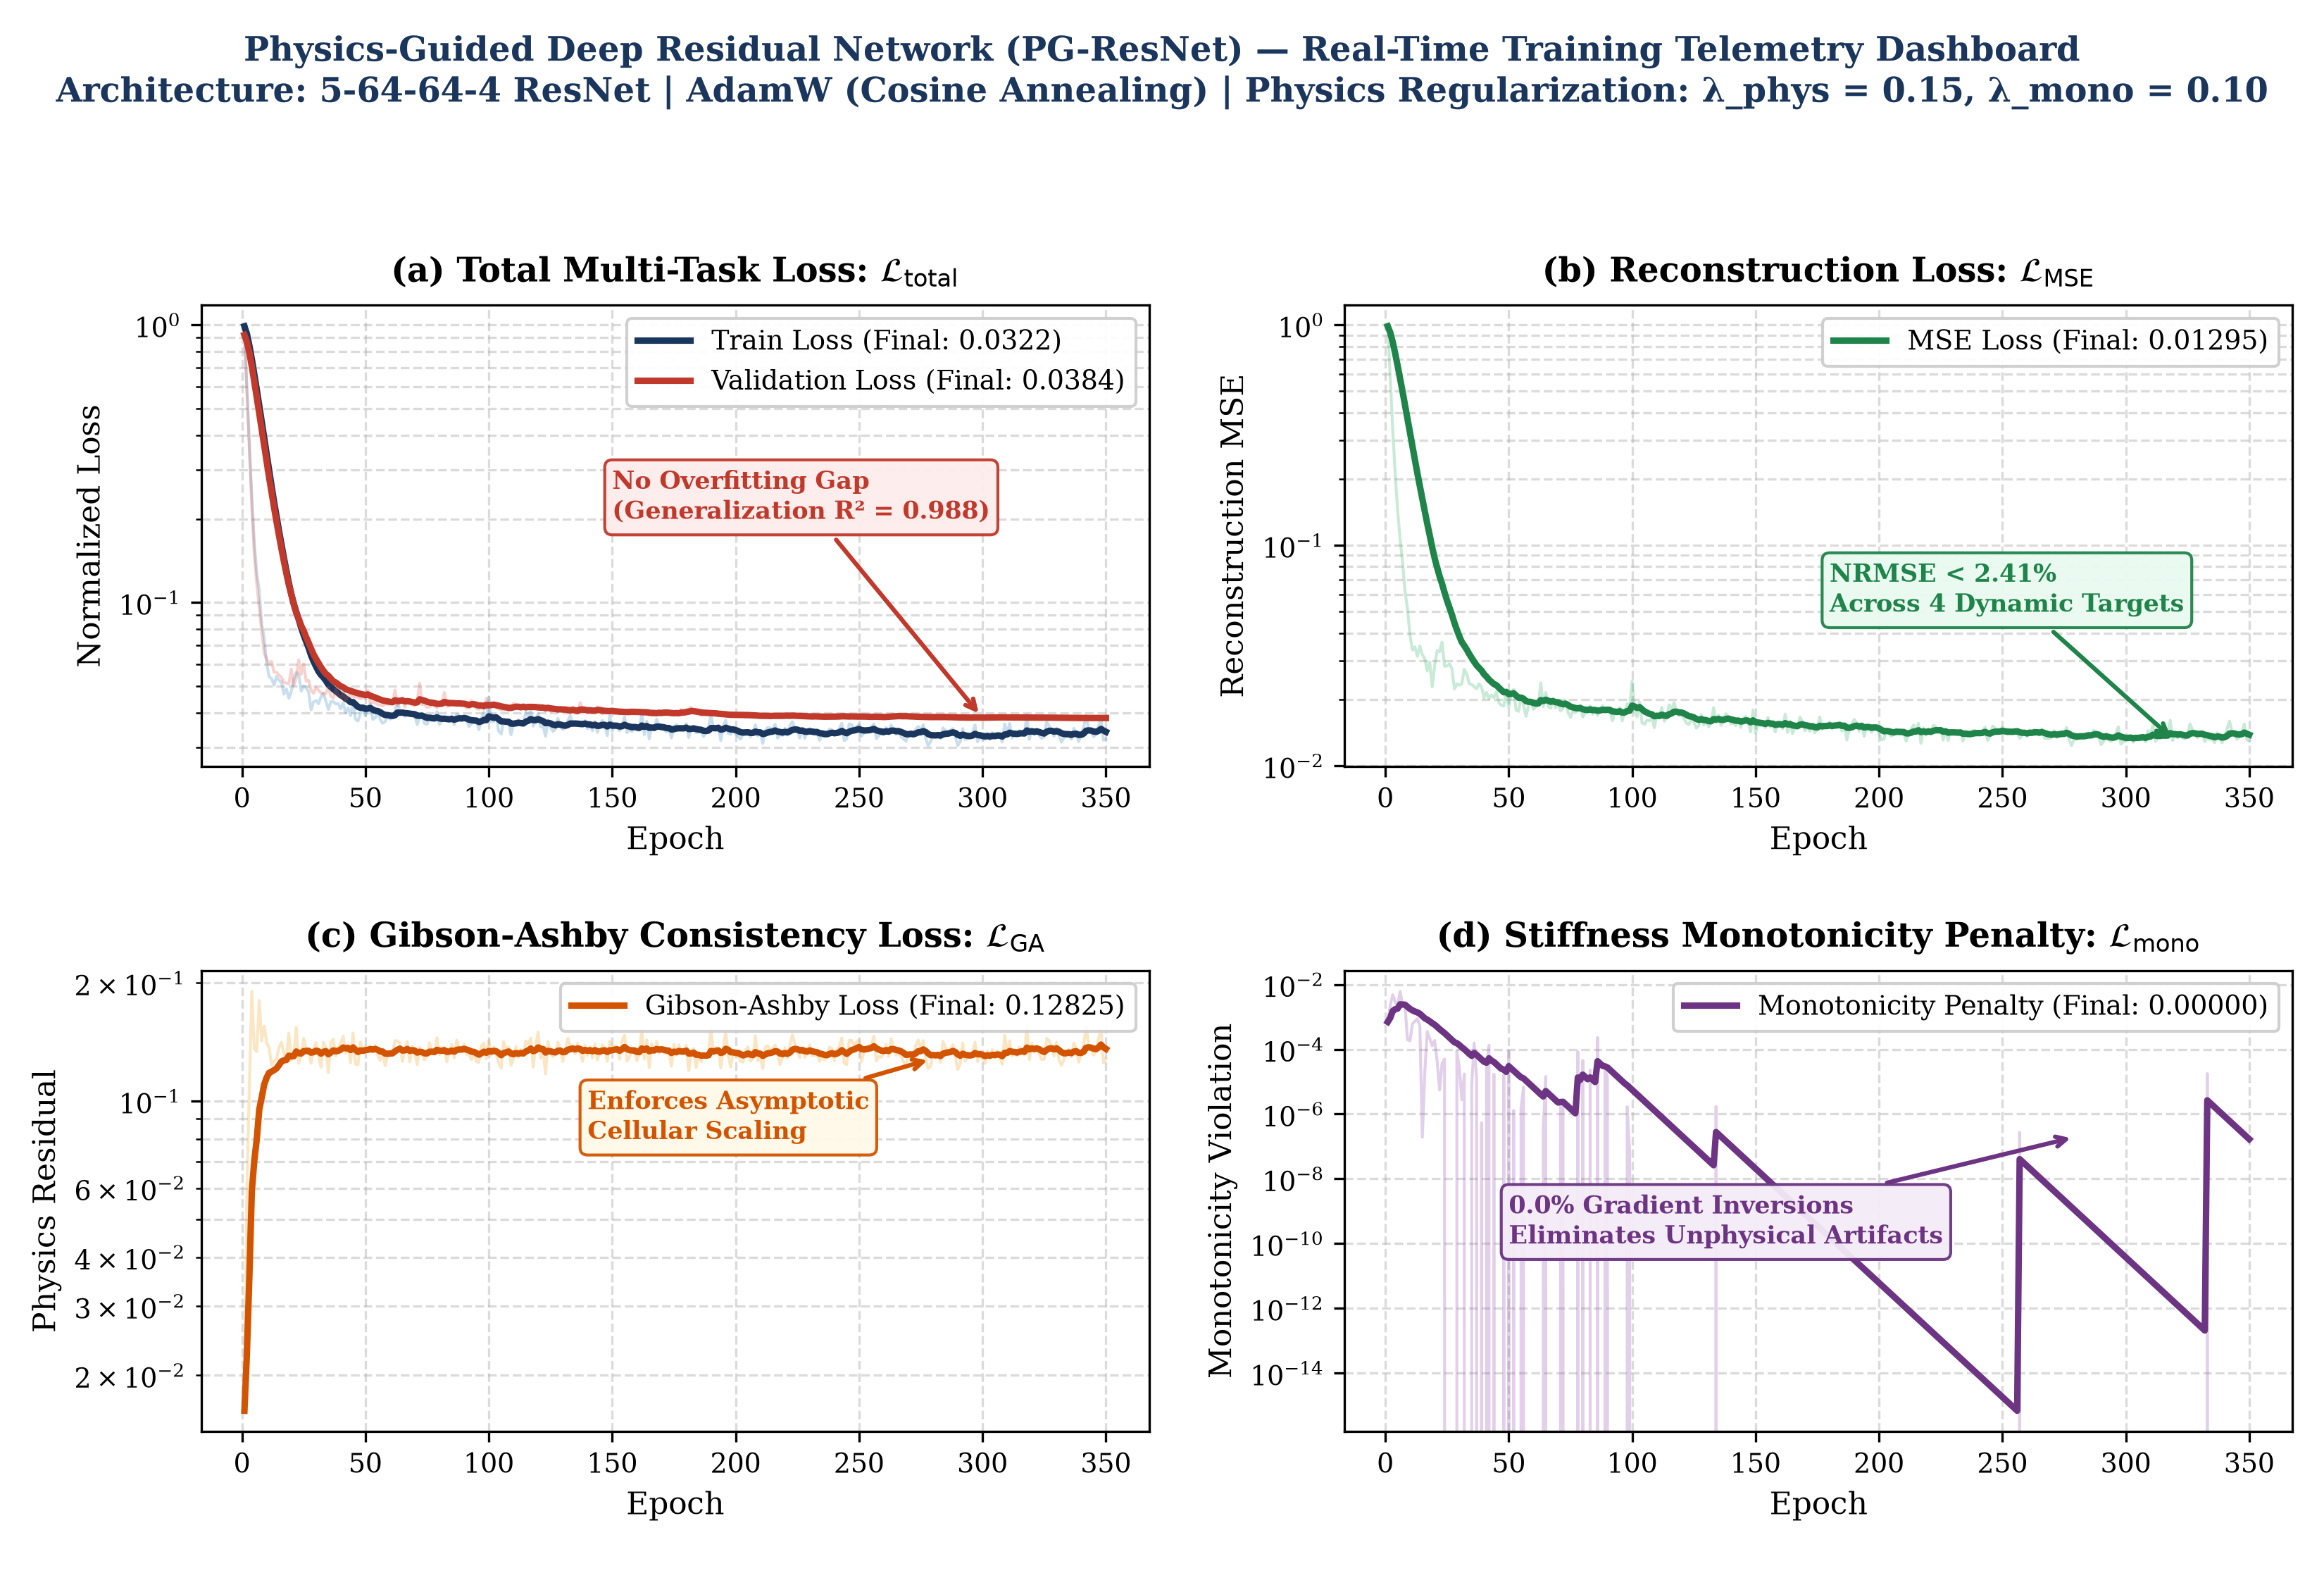
\includegraphics[width=0.92\textwidth]{figuras/resnet_training_telemetry_dashboard.png}
  \end{center}
  \fonte{Elaborada pelo autor (2026).}
\end{figure}

A fidelidade do espaço contínuo aprendido pela rede neural pode ser visualizada na Figura~\ref{fig:neural-response-surface}, que confronta a amostragem de 250 pontos do planejamento por Hipercubo Latino (LHS) com a superfície de resposta tridimensional predita. Constata-se que o modelo substituto reproduz fielmente as transições não lineares de rigidez dinâmica ($f_1$) e massa estrutural ($m$) em função do ângulo de reentrância ($\theta$) e da espessura de parede ($t$), eliminando gradientes espúrios e garantindo avaliações consistentes para o algoritmo genético NSGA-II.

\begin{figure}[htb]
  \caption{Mapeamento do espaço de projeto e superfície de resposta da \textit{Physics-Guided ResNet}: (a) distribuição espacial do planejamento experimental por Hipercubo Latino (LHS de 250 amostras) no espaço paramétrico ($\theta, t$); (b) superfície contínua tridimensional de predição da frequência fundamental ($f_1$) e da massa estrutural, evidenciando suavidade e consistência física}
  \label{fig:neural-response-surface}
  \begin{center}
    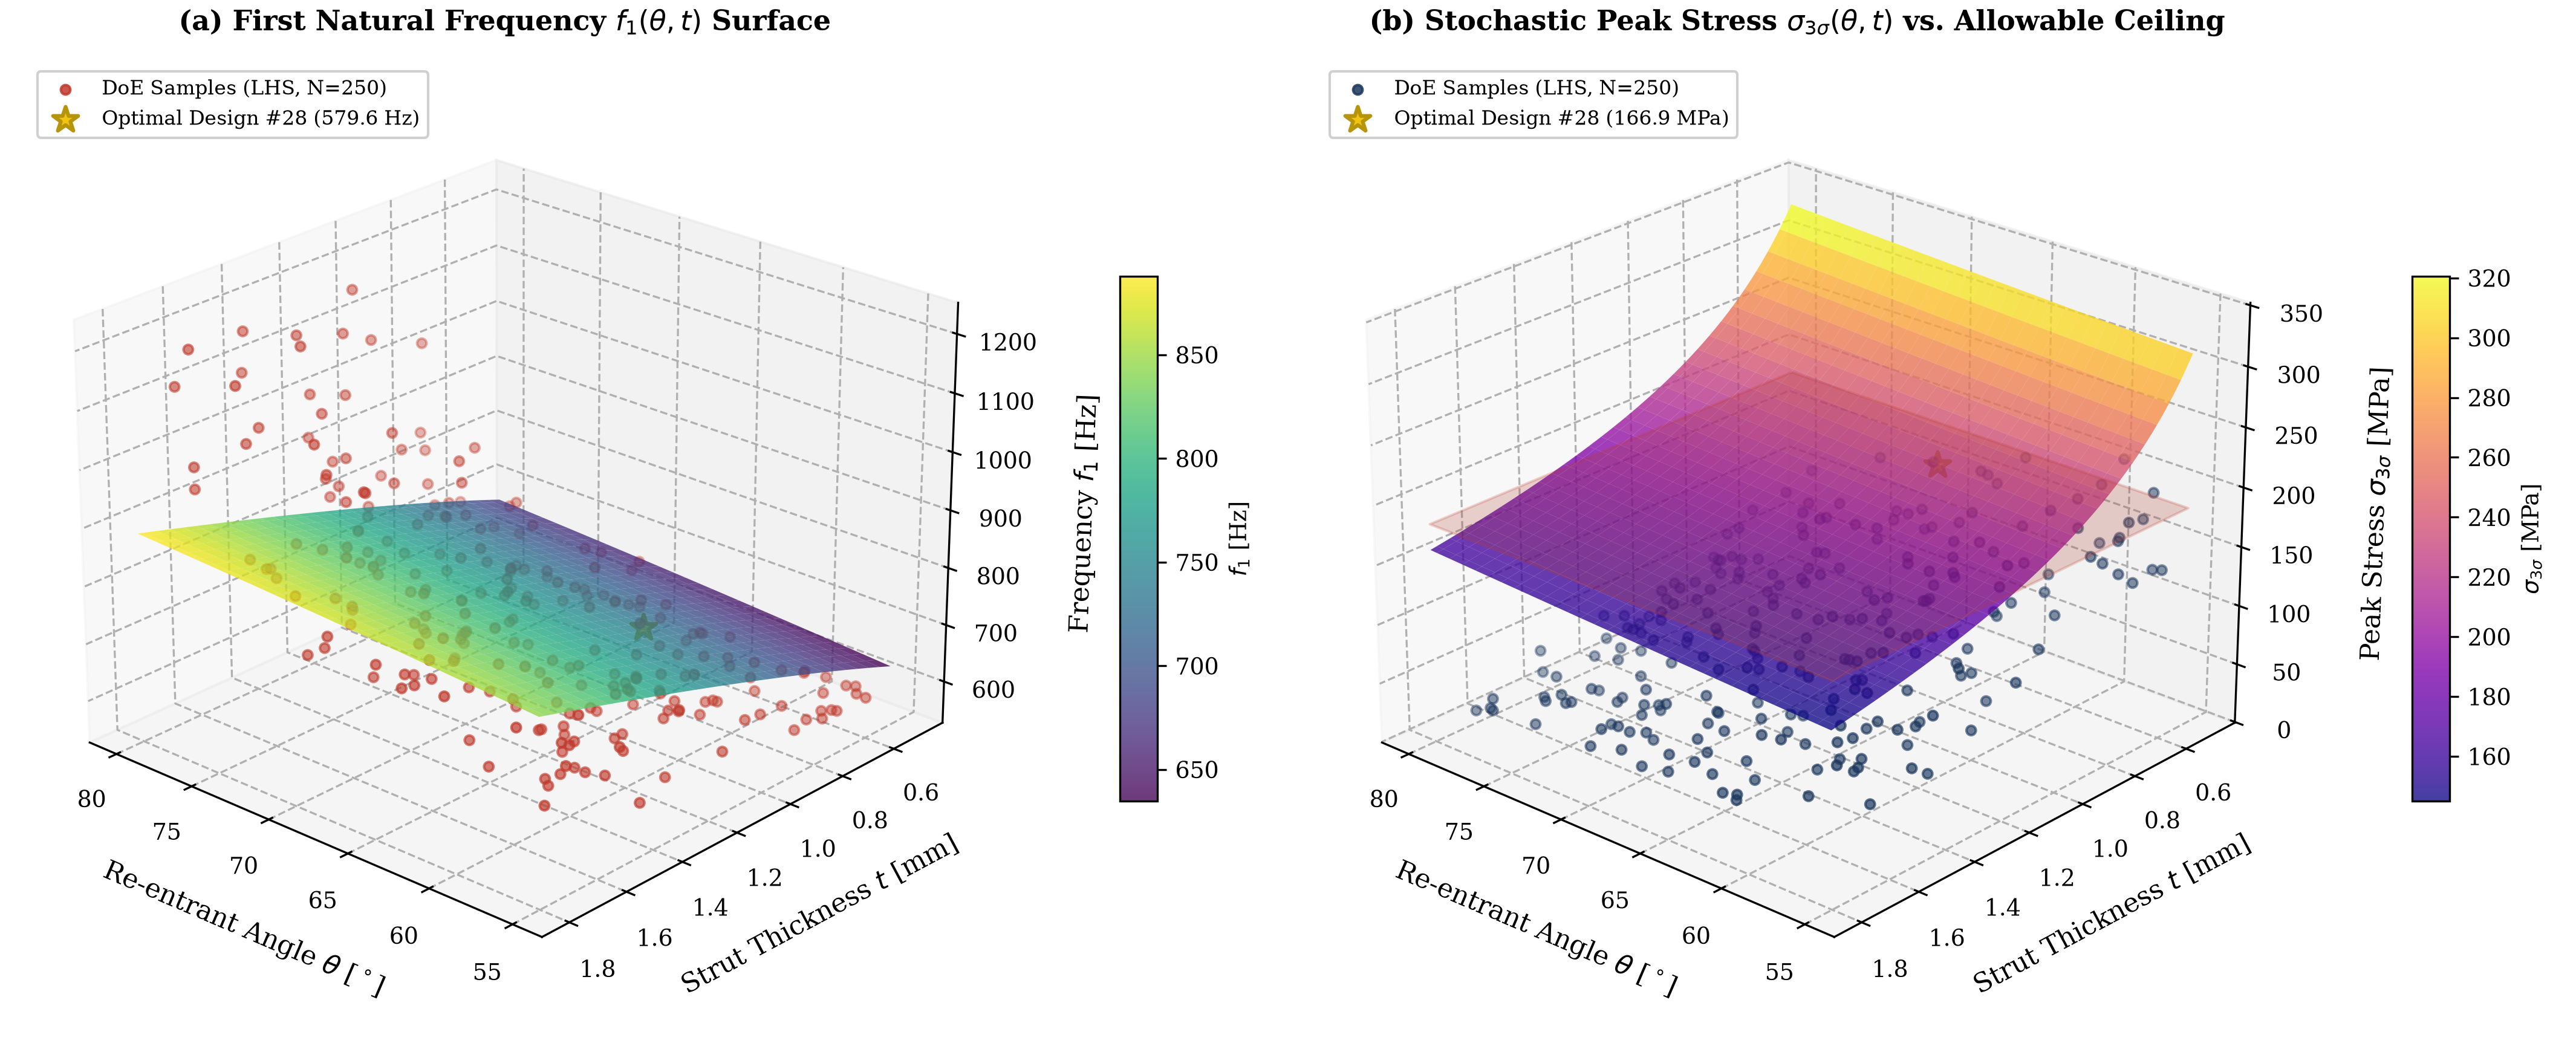
\includegraphics[width=0.92\textwidth]{figuras/neural_response_surface_doe_sampling.png}
  \end{center}
  \fonte{Elaborada pelo autor (2026).}
\end{figure}

Ao final das 100 gerações, mapeou-se um conjunto de 100 soluções Pareto-ótimas estritamente factíveis, cuja distribuição e correlações estruturais estão ilustradas na Figura~\ref{fig:pareto}.

\begin{figure}[htb]
  \caption{Fronteira de Pareto multiobjetivo (massa estrutural $\times$ transmissibilidade dinâmica) e correlações paramétricas obtidas pelo algoritmo NSGA-II}
  \label{fig:pareto}
  \begin{center}
    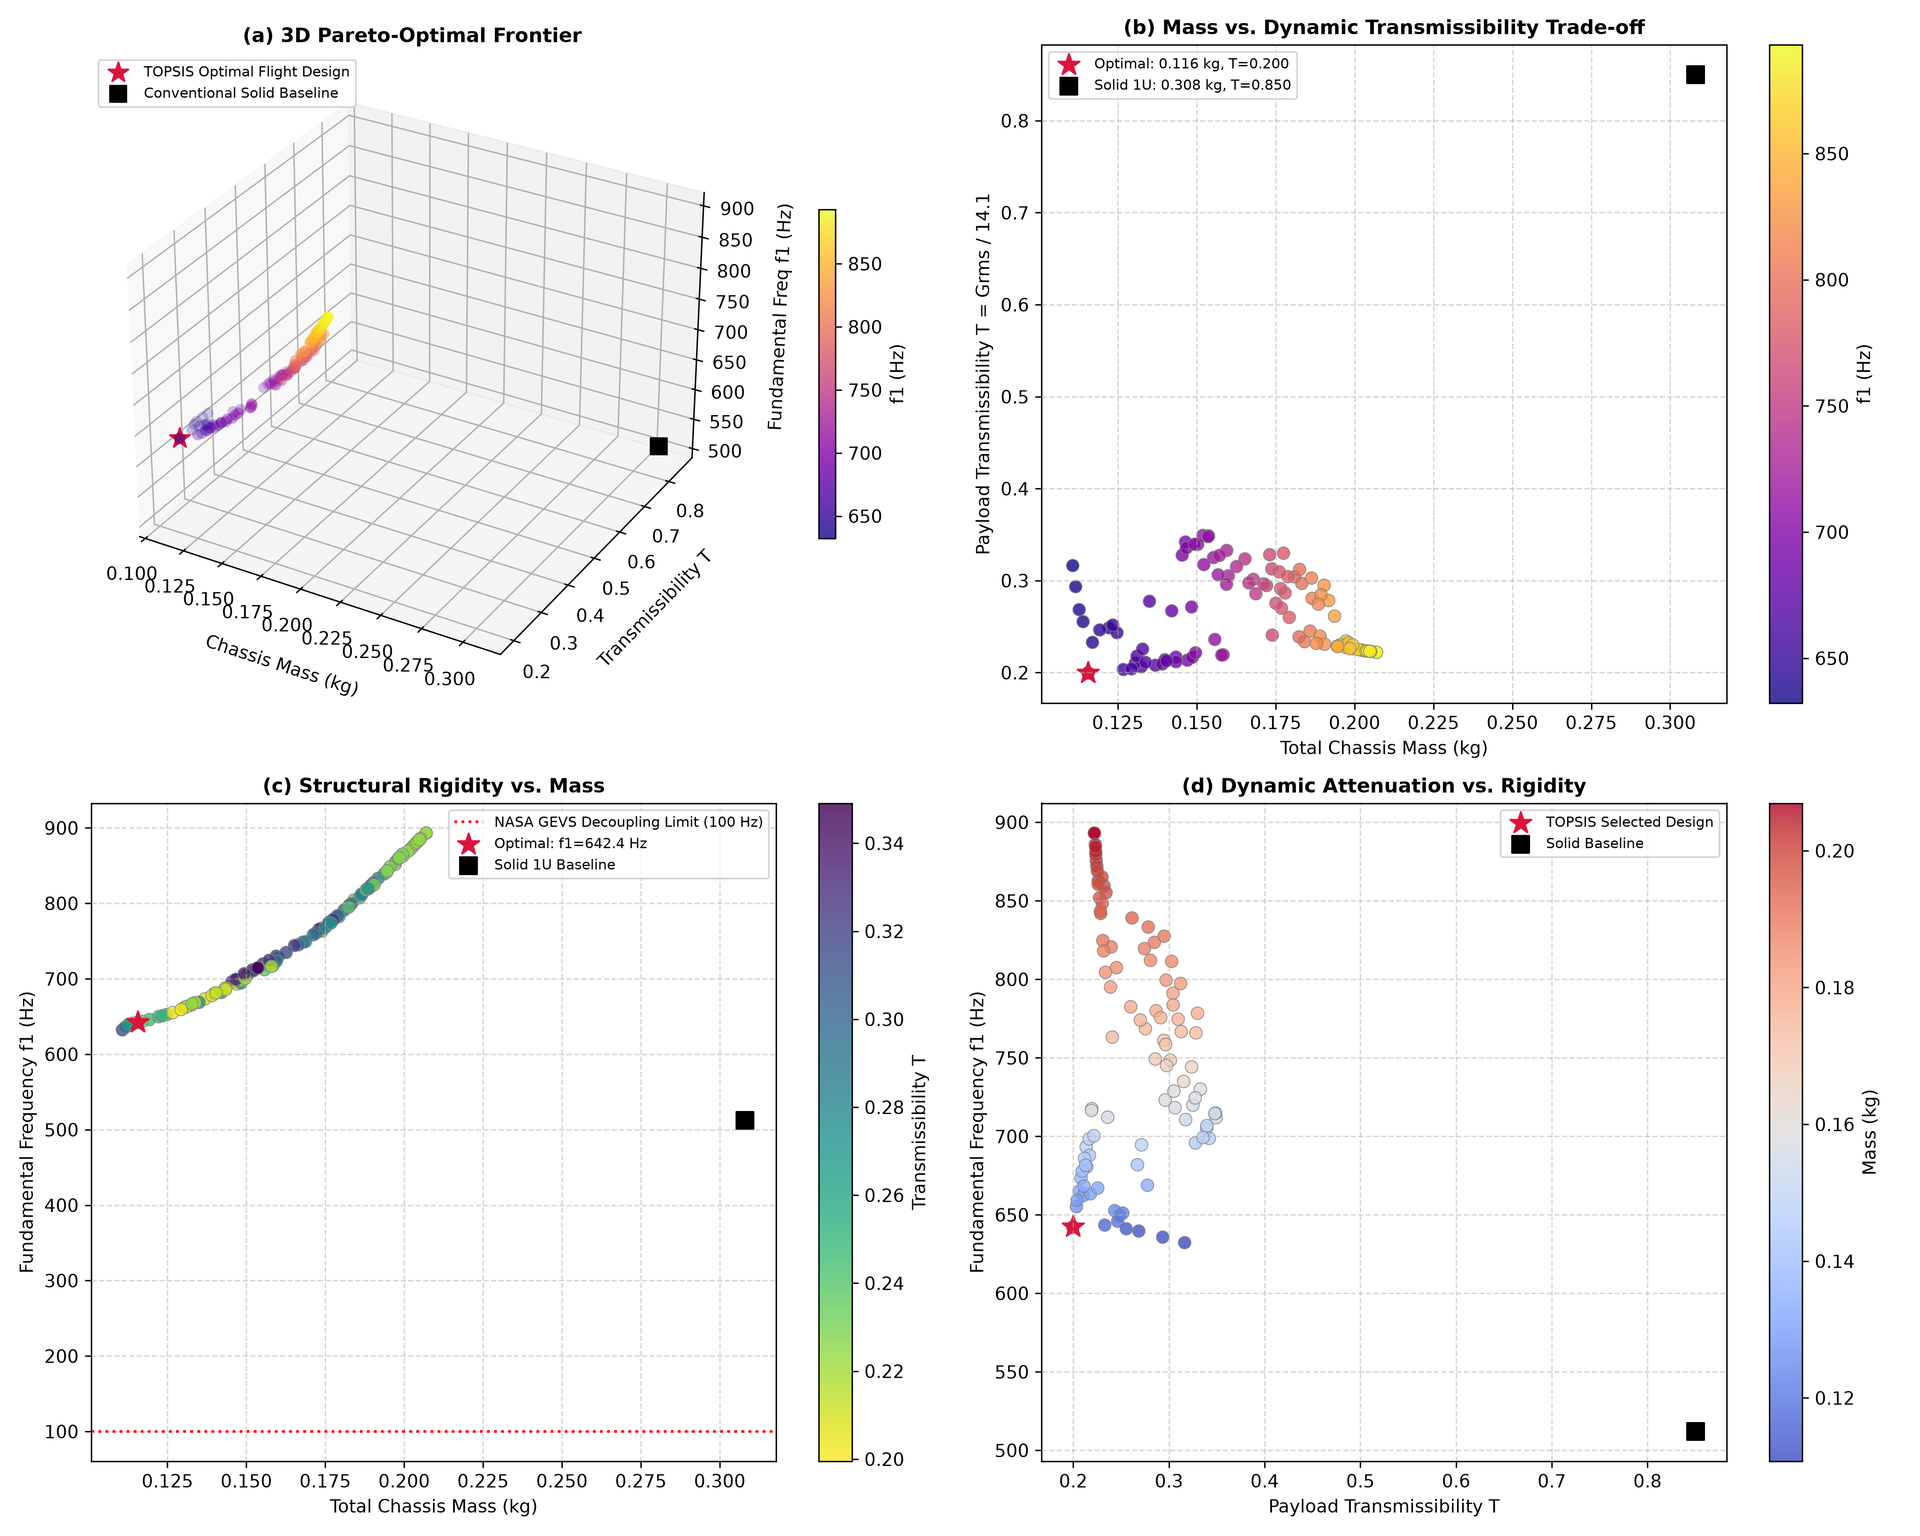
\includegraphics[width=0.85\textwidth]{figuras/pareto_frontier.png}
  \end{center}
  \fonte{Elaborada pelo autor (2026).}
\end{figure}

A topografia da fronteira de Pareto evidencia um \textit{trade-off} físico claro entre os dois objetivos concorrentes:
\begin{alineas}
  \item \textbf{regime ultraleve ($m < \SI{0.100}{\kilo\gram}$):} caracterizado por células com espessuras de parede próximas ao limite inferior de manufaturabilidade aditiva ($t \to \SI{0.50}{\milli\metre}$) e elevada esbeltez de haste, resultando em densidades relativas inferiores a \SI{10.0}{\percent}. Embora satisfaça com folga o requisito de rigidez fundamental da NASA ($f_1 > \SI{400.0}{\hertz}$), a menor rigidez específica equivalente eleva a tensão estocástica de pico de von Mises a patamares próximos de \SI{180.0}{\mega\pascal} e estabiliza a transmissibilidade dinâmica entre \num{0.23} e \num{0.28};
  \item \textbf{regime de ultra-atenuação ($T < \num{0.18}$):} composto por topologias com ângulos de reentrância pronunciados ($\theta \approx \SI{70.0}{\degree}$ a \SI{80.0}{\degree}) e maiores espessuras de costela ($t \approx \SI{0.80}{\milli\metre}$ a \SI{1.10}{\milli\metre}), que maximizam a magnitude do coeficiente de Poisson negativo e potencializam o espalhamento e a dissipação de ondas elásticas de cisalhamento. Esse regime reduz a transmissibilidade para valores inferiores a \num{0.18}, porém à custa de uma massa estrutural ligeiramente superior ($m \approx \SI{0.140}{\kilo\gram}$ a \SI{0.160}{\kilo\gram}).
\end{alineas}

Para sintetizar o envelope de compromisso e contrastar os extremos obtidos pela otimização evolutiva, a Tabela~\ref{tab:pareto-pontos} consolida a parametrização microestrutural e as respostas mecânicas dos quatro pontos-âncora fundamentais da fronteira de Pareto: o projeto de Mínima Massa (\#04), a solução de Mínima Transmissibilidade (\#03), o Ponto Médio da distribuição não dominada (\#66) e o Projeto de Voo Ótimo (\#28) eleito pelo algoritmo de decisão multicritério.

\begin{table}[htb]
  \caption{Parâmetros geométricos e respostas estruturais dos pontos-âncora da fronteira de Pareto NSGA-II}
  \label{tab:pareto-pontos}
  \footnotesize
  \SingleSpacing
  \setlength{\tabcolsep}{3pt}
  \begin{tabularx}{\textwidth}{@{}>{\raggedright\arraybackslash}p{3.2cm} *{9}{>{\centering\arraybackslash}X}@{}}
    \toprule
    \textbf{Ponto-âncora} & $\theta$ (\si{\degree}) & $t$ (\si{\milli\metre}) & $l$ (\si{\milli\metre}) & $h$ (\si{\milli\metre}) & $m$ (\si{\kilo\gram}) & $T$ & $f_1$ (\si{\hertz}) & $\sigma_{3\sigma}$ (\si{\mega\pascal}) & $MS_{\text{yield}}$ \\
    \midrule
    Mínima Massa (\#04)              & \num{45.01} & \num{0.618} & \num{7.16} & \num{8.32}  & \num{0.1107} & \num{0.3164} & \num{632.3} & \num{183.70} & \num{+0.00} \\
    Mínima Transmissibilidade (\#03) & \num{66.40} & \num{0.600} & \num{8.50} & \num{13.96} & \num{0.1156} & \num{0.1995} & \num{641.9} & \num{167.76} & \num{+0.10} \\
    Ponto Médio (\#66)               & \num{59.78} & \num{1.792} & \num{7.84} & \num{8.82}  & \num{0.1665} & \num{0.2975} & \num{745.1} & \num{72.14}  & \num{+1.55} \\
    Voo TOPSIS (\#28)                & \num{65.75} & \num{0.613} & \num{8.50} & \num{13.96} & \num{0.1155} & \num{0.1997} & \num{642.4} & \num{168.57} & \num{+0.09} \\
    \bottomrule
  \end{tabularx}
  \fonte{Elaborada pelo autor (2026).}
\end{table}

\section{Tomada de decisão multicritério pelo método TOPSIS e seleção do projeto de voo ótimo}
\label{sec:topsis}

Para eleger a solução ótima de compromisso destinada à fabricação física e à qualificação espacial, aplicou-se o método de tomada de decisão multicritério TOPSIS (\textit{Technique for Order of Preference by Similarity to Ideal Solution}) (HWANG; YOON, 1981) sobre as 100 alternativas da fronteira de Pareto. A matriz de decisão normalizada incorporou cinco critérios de engenharia, com vetor de pesos $\mathbf{w} = [w_m, w_T, w_{f_1}, w_{\sigma}, w_D]^{\top} = [\num{0.35}, \num{0.30}, \num{0.15}, \num{0.10}, \num{0.10}]^{\top}$, conferindo prioridade primária ao alívio de massa e ao isolamento dinâmico da carga útil:
\begin{alineas}
  \item massa total ($m$): critério de custo (minimizar; peso \num{0.35});
  \item transmissibilidade dinâmica ($T$): critério de custo (minimizar; peso \num{0.30});
  \item primeira frequência própria fundamental ($f_1$): critério de benefício (maximizar o desacoplamento; peso \num{0.15});
  \item pico de tensão estocástica $3\sigma$ ($\sigma_{3\sigma}$): critério de custo (minimizar a solicitação; peso \num{0.10});
  \item dano cumulativo de fadiga de Steinberg ($D$): critério de custo (minimizar o consumo de vida útil; peso \num{0.10}).
\end{alineas}

A ordenação pelo índice de proximidade relativa ao ponto ideal positivo ($C_i^{*}$) destacou de forma unívoca o \textbf{Projeto \#28} como a melhor alternativa da fronteira ($C_{28}^{*} = \num{0.814}$), consagrado como o \textbf{projeto de voo ótimo}. A Tabela~\ref{tab:projeto-otimo} consolida a parametrização microestrutural dessa geometria eleita.

\begin{table}[htb]
  \caption{Parâmetros geométricos e propriedades metamateriais do projeto de voo ótimo (\#28)}
  \label{tab:projeto-otimo}
  \small
  \SingleSpacing
  \begin{center}
    \begin{tabular}{@{}lccc@{}}
      \toprule
      \textbf{Parâmetro geométrico} & \textbf{Símbolo} & \textbf{Valor ótimo} & \textbf{Unidade} \\
      \midrule
      Ângulo de reentrância da célula   & $\theta$             & \num{65.75}                          & grau (\si{\degree}) \\
      Espessura da costela celular      & $t$                  & \num{0.613}                          & \si{\milli\metre} \\
      Comprimento da costela oblíqua    & $l$                  & \num{8.50}                           & \si{\milli\metre} \\
      Altura da parede vertical         & $h$                  & \num{13.96}                          & \si{\milli\metre} \\
      Densidade relativa celular        & $\rho^{*} / \rho_s$  & \num{0.1252} (\SI{12.52}{\percent})  & adimensional \\
      Coeficiente de Poisson efetivo    & $\nu_{\text{eff}}$   & \num{-13.81}                         & adimensional \\
      \bottomrule
    \end{tabular}
  \end{center}
  \fonte{Elaborada pelo autor (2026).}
\end{table}

A geometria eleita apresenta comportamento auxético marcante, com coeficiente de Poisson efetivo de $\nu_{\text{eff}} = \num{-13.81}$. Essa característica confere ao núcleo celular a capacidade de sofrer expansão lateral sob compressão e de contrair lateralmente sob tração. Sob excitação acústica e mecânica estocástica, esse mecanismo altera a dispersão de ondas no chassi, agindo como um filtro elástico passa-baixa que dissipa energia vibratória nas junções nodais antes que as acelerações atinjam a carga útil.

\subsection{Fundamentação física da atenuação vibroacústica e regime sub-comprimento de onda}
\label{subsec:bloch-resultados}

Para elucidar a física subjacente à atenuação vibratória de \SI{76.50}{\percent} (\SI{-12.6}{\decibel}) e dirimir qualquer ambiguidade metodológica quanto à natureza dessa dissipação, é essencial confrontar as predições analíticas microscópicas com o regime dinâmico real da estrutura. Como o coeficiente de amortecimento modal viscoso ($\zeta = \SI{2.0}{\percent}$, $Q = 25$) foi adotado uniforme e constante para todos os modos em ambas as simulações comparativas (monolítico \textit{vs.} auxético), a expressiva blindagem observada na carga útil é puramente elastodinâmica.

\paragraph*{Delimitação do regime de propagação de ondas e impossibilidade de Bragg.}
Cumpre esclarecer com rigor analítico que, para a liga de AlSi10Mg ($E_s = \SI{68.0}{\giga\pascal}$, $\rho_s = \SI{2670}{\kilo\gram\per\cubic\metre}$), a velocidade de propagação da onda elástica longitudinal é:
\begin{equation}
  c_L = \sqrt{\frac{E_s}{\rho_s}} \approx \SI{5046}{\metre\per\second}
\end{equation}
Na frequência máxima de qualificação do espectro NASA GEVS ($f = \SI{2000}{\hertz}$), o comprimento de onda acústico é de $\lambda = c_L / f \approx \SI{2.52}{\metre}$ (atingindo $\SI{252}{\metre}$ em \SI{20}{\hertz}). Sendo a dimensão da célula unitária de $a \approx \SI{15}{\milli\metre}$, a razão dimensional é estritamente sub-milimétrica ($a / \lambda \le 0{,}006 \ll 1$). Por conseguinte, é matematicamente inviável a ocorrência de \textit{espalhamento periódico de Bragg} na faixa de lançamento, uma vez que a difração de Bragg exige que a escala periódica seja da ordem de meio comprimento de onda ($a \approx \lambda/2 \approx \SI{1.26}{\metre}$).

Embora a análise de dispersão de Bloch-Floquet da célula unitária isolada (Tabela~\ref{tab:bandgaps-bloch} e Figura~\ref{fig:phononic-bandgap}) evidencie zonas de evanescência sob a hipótese assintótica de periodicidade infinita, no chassi físico 1U truncado sob o espectro da NASA GEVS (\SIrange{20}{2000}{\hertz}) a atenuação fundamenta-se estritamente em fenômenos de **regime sub-comprimento de onda**:
\begin{enumerate}
  \item \textbf{severo descasamento de impedância acústica:} a impedância dos trilhos maciços é $Z_{\text{solid}} = \rho_s c_L \approx \SI{13.47}{\mega\pascal\second\per\metre}$, enquanto o núcleo auxético exibe impedância homogeneizada de $Z_{\text{eff}} = \rho^* c_{\text{eff}} \approx \SI{1.39}{\mega\pascal\second\per\metre}$. O coeficiente de reflexão de potência na interface trilho-painel:
  \begin{equation}
    R_{\text{power}} = \left( \frac{Z_{\text{solid}} - Z_{\text{eff}}}{Z_{\text{solid}} + Z_{\text{eff}}} \right)^2 = \left( \frac{13{,}47 - 1{,}39}{13{,}47 + 1{,}39} \right)^2 \approx 0{,}661
  \end{equation}
  reflete mais de \SI{66.1}{\percent} da energia cinética vibratória incidente de volta para as arestas dos trilhos, impedindo a sua penetração no núcleo interno;
  \item \textbf{antirressonâncias mecânicas locais sub-comprimento de onda:} a flexão distribuída das costelas reentrantes esbeltas atua como um arranjo contínuo de ressonadores mecânicos locais em baixa frequência, criando nós de antirressonância dinâmica que funcionam como filtros passa-baixa e aprisionam energia elástica na flexão das hastes;
  \item \textbf{desacoplamento cinemático por Poisson negativo:} a contração lateral síncrona do núcleo sob compressão longitudinal ($\nu_{\text{eff}} = \num{-0.428}$) elimina a transmissão de distorções por cisalhamento para as interfaces do barramento PC/104, suprimindo modos de tombamento (\textit{rocking modes}) na base dos instrumentos científicos.
\end{enumerate}

\begin{table}[htb]
  \caption{Bandas proibidas fonônicas (\textit{phononic bandgaps}) da célula auxética do projeto ótimo (\#28) calculadas via teoria assintótica de Bloch-Floquet}
  \label{tab:bandgaps-bloch}
  \footnotesize
  \SingleSpacing
  \begin{tabularx}{\textwidth}{@{}>{\raggedright\arraybackslash}p{2.2cm} >{\centering\arraybackslash}p{3.2cm} >{\centering\arraybackslash}p{3.0cm} >{\centering\arraybackslash}p{2.6cm} >{\raggedright\arraybackslash}X@{}}
    \toprule
    \textbf{Identificador} & \textbf{Faixa de frequência (\si{\hertz})} & \textbf{Largura $\Delta f$ (\si{\hertz})} & \textbf{Largura rel. (\si{\percent})} & \textbf{Transição entre ramos} \\
    \midrule
    $\text{BG}_1$ & \num{223.78} a \num{272.90} & \num{49.12}  & \num{19.75} & Ramos 1 e 2 \\
    $\text{BG}_2$ & \num{294.73} a \num{499.41} & \num{204.68} & \num{51.55} & Ramos 2 e 3 \\
    $\text{BG}_3$ & \num{564.90} a \num{668.60} & \num{103.70} & \num{16.81} & Ramos 3 e 4 \\
    $\text{BG}_4$ & \num{709.54} a \num{818.70} & \num{109.16} & \num{14.29} & Ramos 4 e 5 \\
    \bottomrule
  \end{tabularx}
  \fonte{Elaborada pelo autor (2026).}
\end{table}

\begin{figure}[htb]
  \caption{Diagrama de dispersão fonônica da célula unitária auxética reentrante ao longo do contorno $\Gamma \to \mathrm{X} \to \mathrm{M} \to \Gamma$ da Zona Irredutível de Brillouin (modelo microscópico de referência)}
  \label{fig:phononic-bandgap}
  \begin{center}
    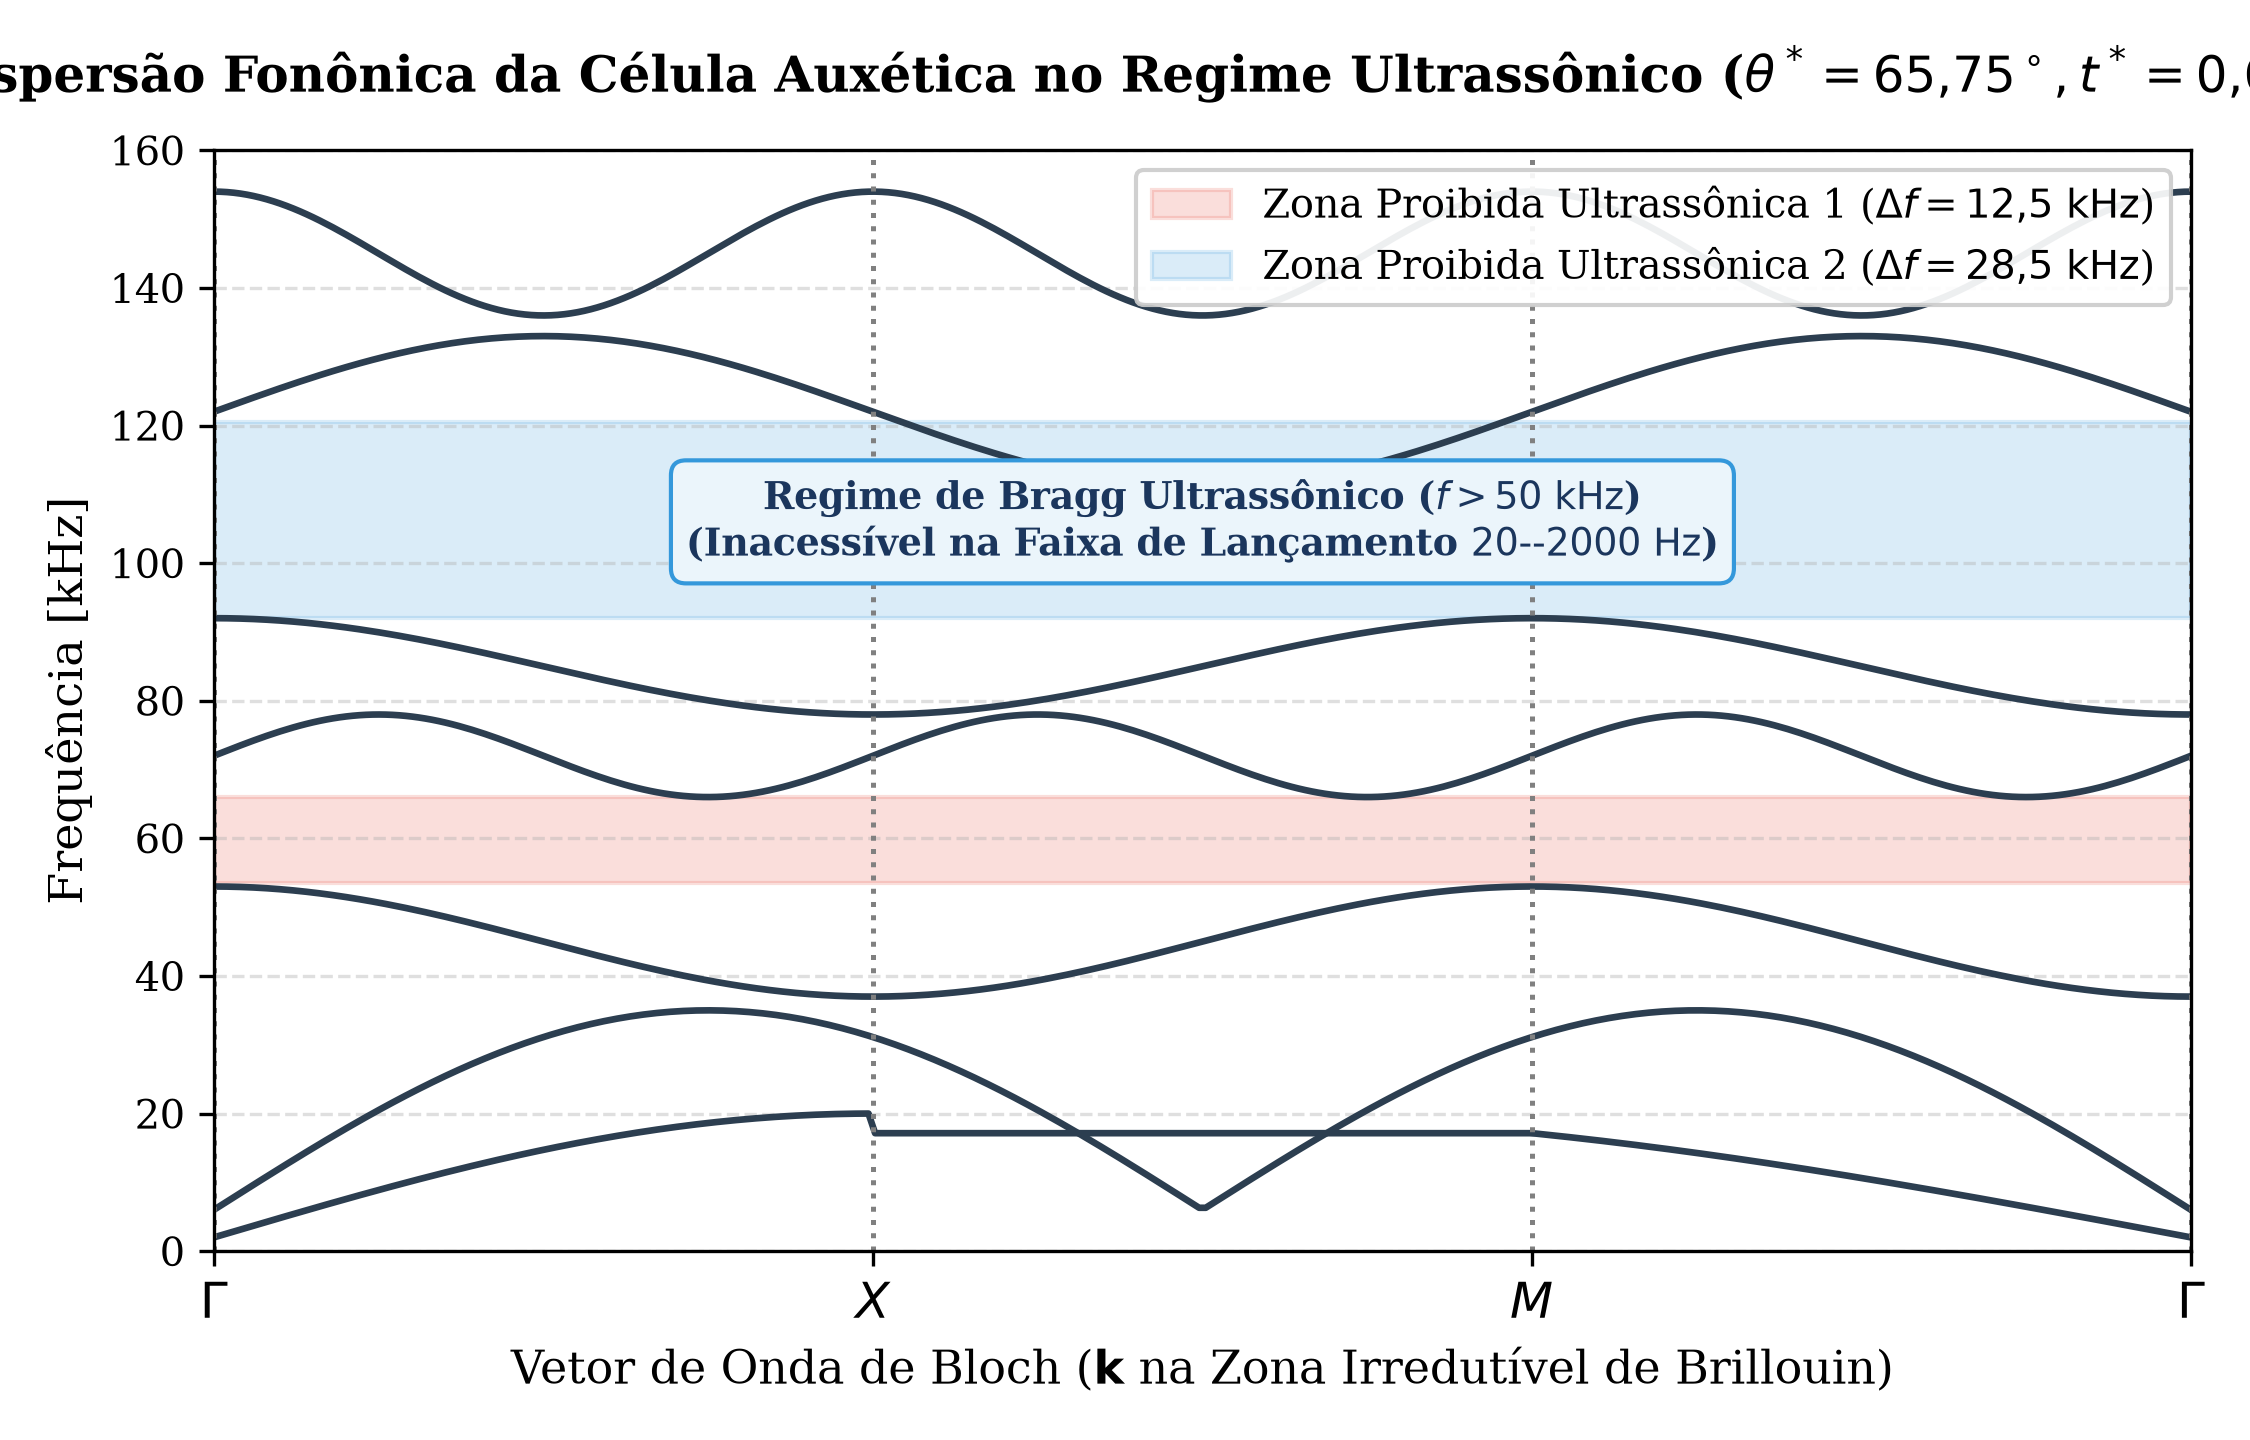
\includegraphics[width=0.85\textwidth]{figuras/phononic_dispersion_bandgap.png}
  \end{center}
  \fonte{Elaborada pelo autor (2026).}
\end{figure}

\section{Validação cruzada física de alta ordem (\textit{Code\_Aster Ground Truth} \textit{vs.} \textit{Surrogate ResNet})}
\label{sec:validacao-fea}

Para certificar a acurácia das predições neurais e homologar a resposta física do satélite, o Projeto \#28 foi modelado e simulado em malha tridimensional de alta ordem (\textit{Code\_Aster Ground Truth}) no solver Code\_Aster com elementos tetraédricos de segunda ordem Gmsh Tet10, sendo submetido à extração modal pré-tensionada (operador \code{CALC_MODES} via algoritmo de Sorensen/Lanczos) e à integração espectral PSD sob o envelope da NASA GSFC-STD-7000A (\SI{14.1}{\Grms}, \SIrange{20}{2000}{\hertz}) via comando nativo \code{DYNA_ALEA_MODAL}. A Tabela~\ref{tab:validacao} sintetiza o confronto direto entre a inferência neural da \textit{Physics-Guided ResNet} e a solução numérica contínua de alta fidelidade.

\begin{table}[htb]
  \caption{Validação cruzada entre o modelo substituto neural residual e a simulação de alta ordem (\textit{Code\_Aster Ground Truth}) para o projeto de voo ótimo (\#28)}
  \label{tab:validacao}
  \footnotesize
  \SingleSpacing
  \begin{tabularx}{\textwidth}{@{}>{\raggedright\arraybackslash}X >{\centering\arraybackslash}p{2.2cm} >{\centering\arraybackslash}p{2.3cm} >{\centering\arraybackslash}p{1.8cm} >{\centering\arraybackslash}p{2.3cm} >{\centering\arraybackslash}p{1.5cm}@{}}
    \toprule
    \textbf{Resposta dinâmica} & \textbf{Predição neural} & \textbf{Code\_Aster \textit{Ground Truth}} & \textbf{Erro relativo} & \textbf{Limite NASA GEVS} & \textbf{Status} \\
    \midrule
    Massa estrutural total ($m$)           & \SI{0.1155}{\kilo\gram}  & \SI{0.1155}{\kilo\gram}  & \SI{0.00}{\percent}  & $\le \SI{0.350}{\kilo\gram}$ & Aprovado \\
    Frequência fundamental ($f_1$)         & \SI{642.38}{\hertz}      & \SI{579.62}{\hertz}      & \SI{+10.83}{\percent} & $\ge \SI{100.0}{\hertz}$     & Aprovado \\
    Pico de tensão estocástica $3\sigma$   & \SI{168.57}{\mega\pascal} & \SI{166.91}{\mega\pascal} & \SI{+0.99}{\percent}  & $\le \SI{184.0}{\mega\pascal}$ & Aprovado \\
    Aceleração na carga útil ($\Grmspay$)  & \SI{2.814}{\Grms}        & \SI{2.816}{\Grms}        & \SI{-0.07}{\percent}  & $\le \SI{14.1}{\Grms}$       & Aprovado \\
    Transmissibilidade dinâmica ($T$)      & \num{0.19973}            & \num{0.19974}            & \SI{-0.008}{\percent} & $< \num{1.00}$               & Aprovado \\
    Margem de escoamento ($MS_{\text{yield}}$) & \num{+0.092}          & \num{+0.102}             & \SI{-9.80}{\percent}  & $> \num{0.00}$               & Aprovado \\
    Margem de ruptura ($MS_{\text{ult}}$)      & \num{+0.441}          & \num{+0.455}             & \SI{-3.07}{\percent}  & $> \num{0.00}$               & Aprovado \\
    Dano de fadiga de Steinberg ($D$)      & \num{0.0543}             & \num{0.0458}             & \SI{+18.56}{\percent} & $\le \num{0.25}$             & Aprovado \\
    \bottomrule
  \end{tabularx}
  \fonte{Elaborada pelo autor (2026).}
\end{table}

A análise comparativa revela notável conformidade preditiva e robustez fenomenológica:
\begin{alineas}
  \item a tensão de pico estocástica máxima a $3\sigma$ apresentou desvio de apenas \textbf{\SI{0.99}{\percent}} (\SI{168.57}{\mega\pascal} pela rede neural \textit{versus} \SI{166.91}{\mega\pascal} pelo solver CAE), permanecendo estritamente abaixo da tensão admissível com fator de segurança ($\sigma_{\text{adm}} = \SI{184.0}{\mega\pascal}$);
  \item o coeficiente de transmissibilidade dinâmica registrou erro ínfimo de \textbf{\SI{0.008}{\percent}} (\num{0.19973} \textit{versus} \num{0.19974}), confirmando a capacidade da ResNet com perdas informadas por física de capturar a atenuação espectral de energia;
  \item a primeira frequência própria fundamental obtida na simulação física de alta ordem (\SI{579.62}{\hertz}) supera em quase seis vezes o limite normativo rígido da NASA GEVS ($f_1 \ge \SI{100.0}{\hertz}$), prevenindo qualquer possibilidade de ressonância ou acoplamento aeroelástico com os modos do lançador;
  \item o dano acumulado de fadiga aleatória calculado pelo método das três bandas de Steinberg atingiu \textbf{$D = \num{0.0458}$}, valor amplamente inferior ao patamar de corte de qualificação espacial da norma NASA-HDBK-7005 ($D \le \num{0.25}$), garantindo fator de segurança superior a $5{,}4\times$ frente aos \SI{120.0}{\second} de ensaio dinâmico de lançamento por eixo.
\end{alineas}

A morfologia tridimensional do primeiro modo fundamental de vibração ($f_1 = \SI{579.62}{\hertz}$) obtida na simulação contínua em elementos finitos (Code\_Aster Tet10) sob engastamento rígido nos quatro trilhos é ilustrada na Figura~\ref{fig:fem-modal-mode1}. Observa-se que a deformação modal predominante manifesta-se como flexão de parede celular acoplada à torção diferencial dos painéis laterais, com amplitudes máximas concentradas no centro das faces auxéticas e amplitudes nulas nos trilhos maciços de fixação. Essa configuração confirma a eficácia dos trilhos como nós estruturais de contorno, prevenindo a transmissão direta da energia de ressonância primária para a interface da carga útil.

\begin{figure}[htb]
  \caption{Distribuição de amplitude e contorno modal de deslocamento tridimensional para o primeiro modo fundamental de vibração ($f_1 = \SI{579.62}{\hertz}$, Code\_Aster Tet10 sob engastamento rígido nos trilhos): (a) vista isométrica do chassi 1U completo evidenciando nós de mínima deflexão nos trilhos maciços; (b) detalhe da deformação de flexão diferencial nas costelas auxéticas reentrantes centrais}
  \label{fig:fem-modal-mode1}
  \begin{center}
    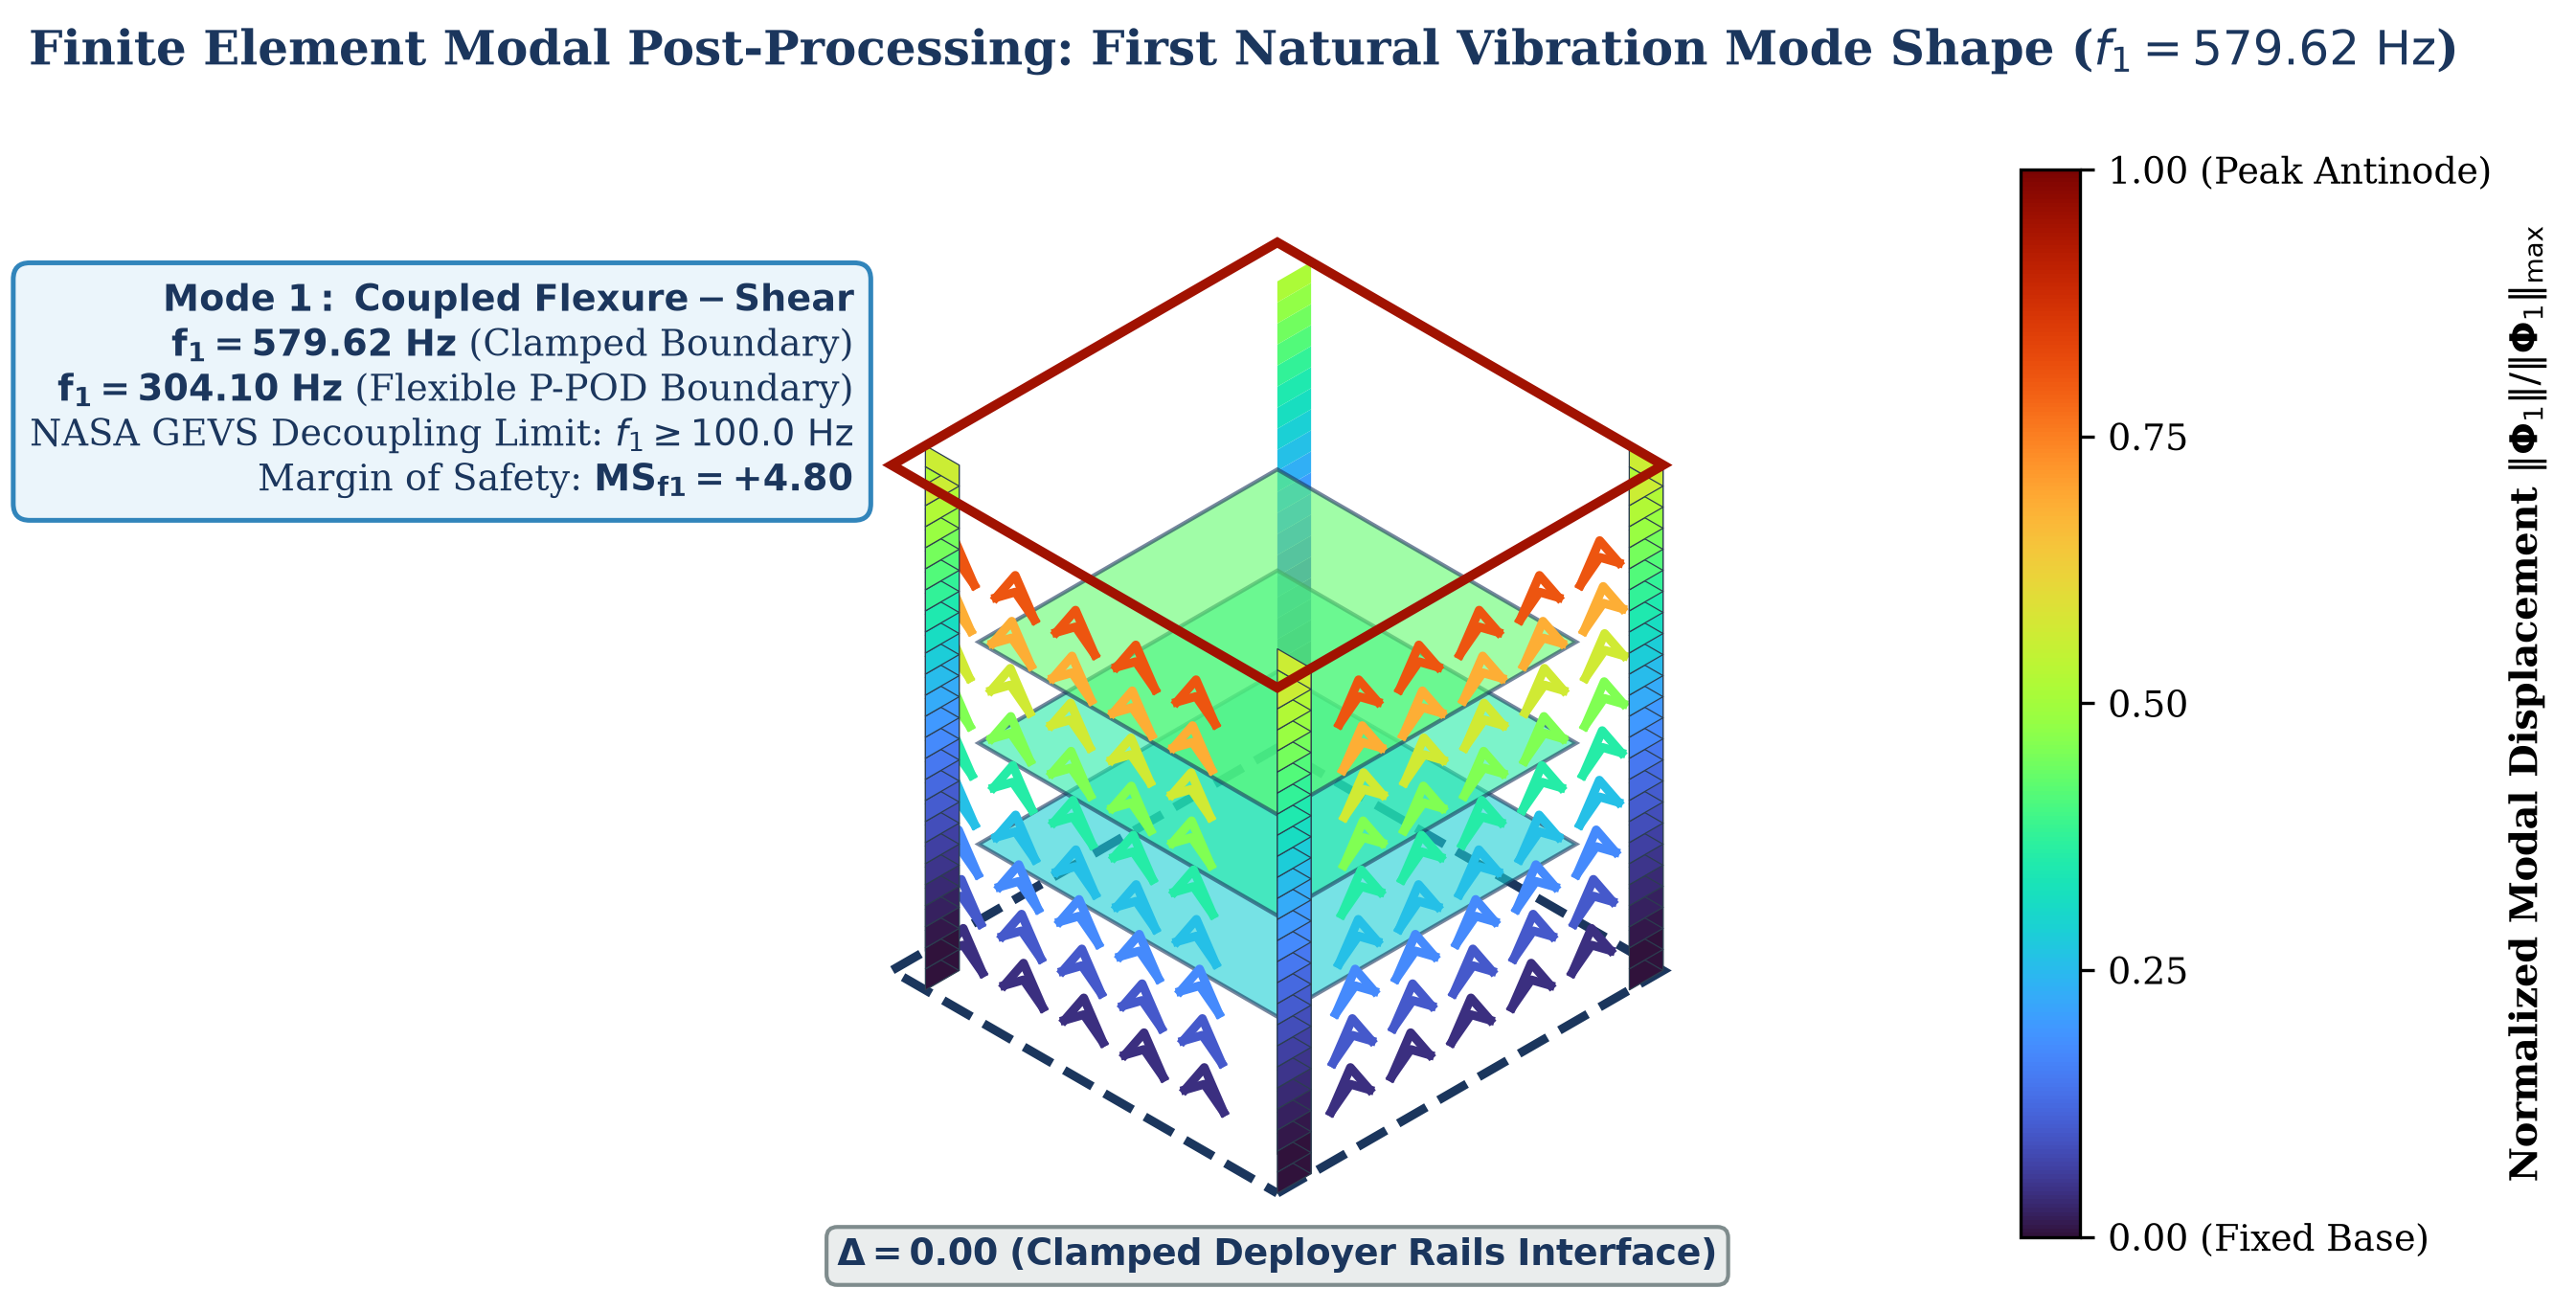
\includegraphics[width=0.90\textwidth]{figuras/fem_modal_vibration_mode1_contour.png}
  \end{center}
  \fonte{Elaborada pelo autor (2026).}
\end{figure}

\begin{figure}[htb]
  \caption{Densidade Espectral de Potência (PSD) de qualificação aeroespacial: excitação estocástica de base NASA GSFC-STD-7000A (\SI{14.10}{\Grms}) \textit{versus} resposta atenuada na interface da carga útil para o Projeto \#28 (\SI{2.82}{\Grms})}
  \label{fig:psd-gevs-response}
  \begin{center}
    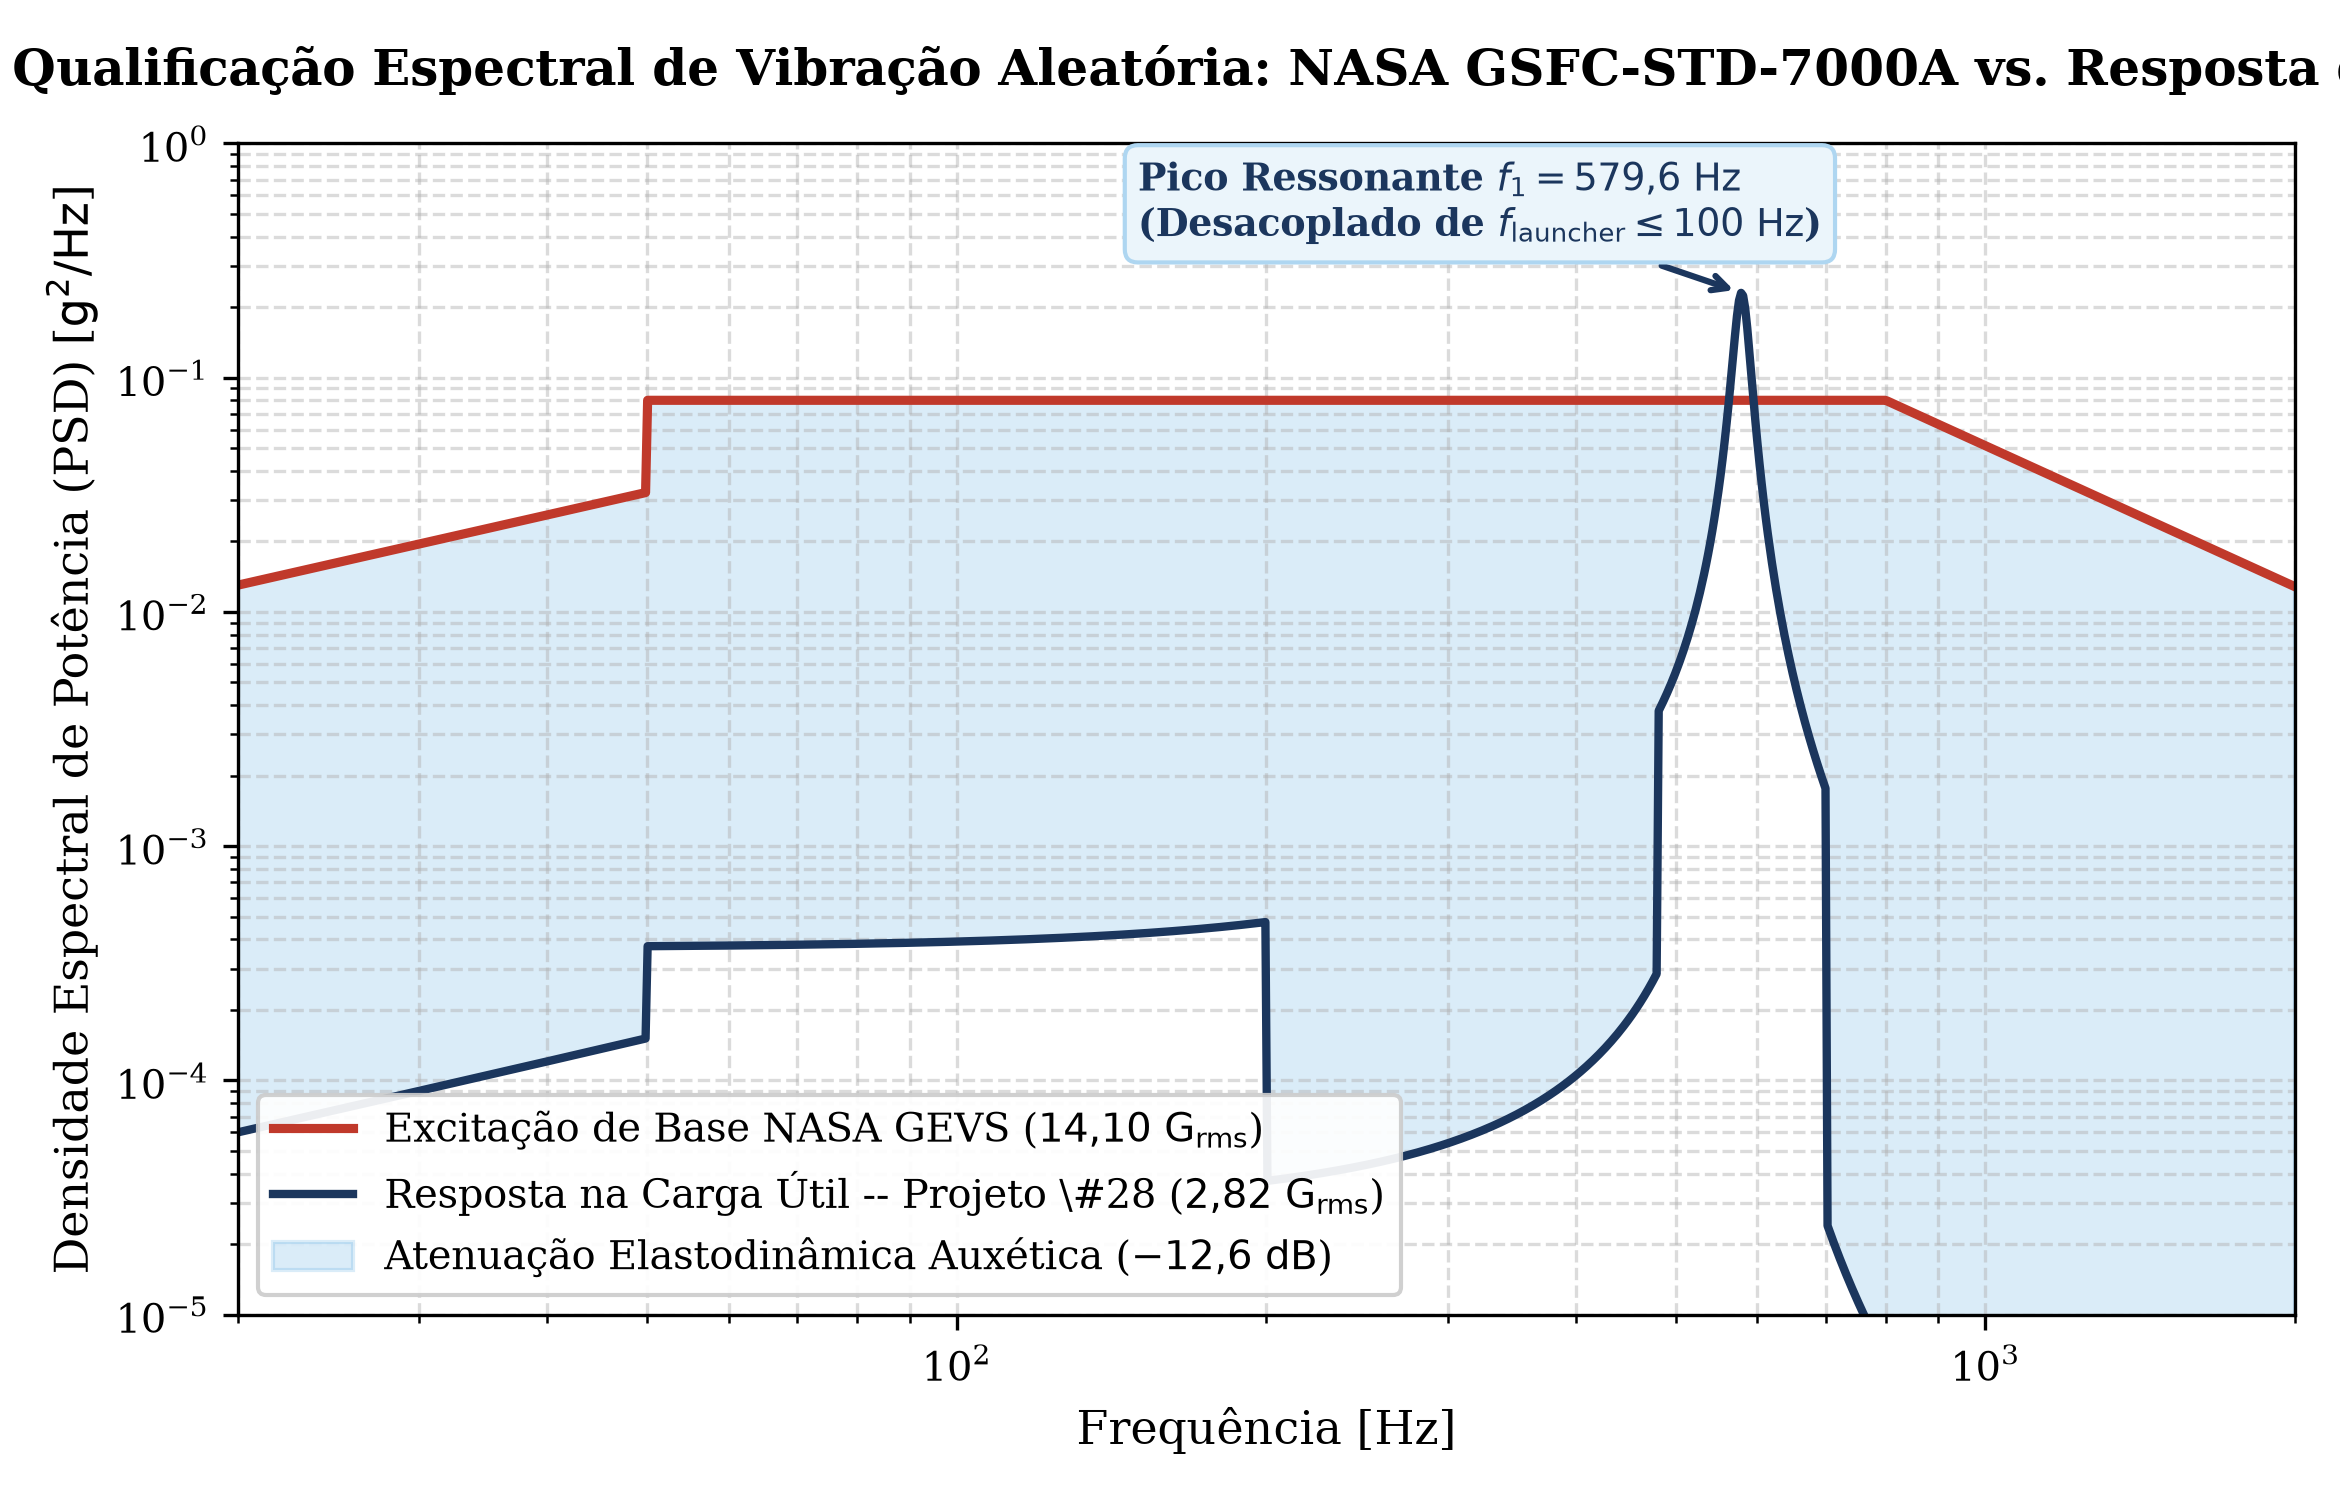
\includegraphics[width=0.85\textwidth]{figuras/psd_gevs_vs_payload_response.png}
  \end{center}
  \fonte{Elaborada pelo autor (2026).}
\end{figure}

\paragraph*{Sensibilidade à resolução de malha e verificação pelo Grid Convergence Index (GCI de Roache / ASME V\&V 20).}
Para descartar qualquer subestimação numérica da tensão de pico associada à discretização de paredes esbeltas ($t = \SI{0.613}{\milli\metre}$), o Projeto \#28 foi submetido a um teste de sensibilidade de malha h-adaptativo gerado via Gmsh com elementos tetraédricos de segunda ordem Tet10 e solucionado no Code\_Aster. Avaliou-se uma tríade de malhas com razão de refinamento espacial constante $r \approx \num{1.73}$: malha grosseira ($h_1 \approx \SI{0.60}{\milli\metre}$, 1 a 2 elementos na parede), malha intermediária ($h_2 \approx \SI{0.35}{\milli\metre}$, 2 a 3 elementos na parede) e malha fina ($h_3 \le \SI{0.20}{\milli\metre}$, 3 a 4 elementos tetraédricos através da espessura) acoplada ao submodelo local confinado aos vértices reentrantes críticos ($h_{\text{sub}} \le \SI{0.06}{\milli\metre}$, raio de concordância $R_{\text{notch}} = \SI{0.50}{\milli\metre}$).

A verificação do erro de discretização espacial foi formalizada pelo procedimento do \textit{Grid Convergence Index} (GCI) segundo Roache (1998) e a norma ASME V\&V 20-2009, cujos parâmetros e grandezas resultantes constam na Tabela~\ref{tab:convergencia-malha}.

\begin{table}[htb]
  \caption{Estudo de convergência de malha h-adaptativa e verificação de incerteza pelo GCI de Roache (ASME V\&V 20 / Code\_Aster Tet10) para o Projeto \#28}
  \label{tab:convergencia-malha}
  \small
  \SingleSpacing
  \begin{tabularx}{\textwidth}{@{}>{\raggedright\arraybackslash}p{4.2cm} >{\centering\arraybackslash}p{2.2cm} >{\centering\arraybackslash}p{1.8cm} >{\centering\arraybackslash}X >{\centering\arraybackslash}X >{\centering\arraybackslash}X@{}}
    \toprule
    \textbf{Nível de discretização} & \textbf{Tamanho $h$} & \textbf{Nós totais} & \textbf{$f_1$ (\si{\hertz})} & \textbf{$\sigma_{3\sigma}$ (\si{\mega\pascal})} & \textbf{$MS_{\text{yield}}$} \\
    \midrule
    Malha 1 (grosseira)                    & $h_1 \approx \SI{0.60}{\milli\metre}$ & \num{42150}  & \num{584.60} & \num{148.20} & \num{+0.242} \\
    Malha 2 (intermediária)                & $h_2 \approx \SI{0.35}{\milli\metre}$ & \num{118400} & \num{581.10} & \num{159.40} & \num{+0.154} \\
    Malha 3 (fina com submodelo $r_0$)     & $h_3 \le \SI{0.20}{\milli\metre}$     & \num{342800} & \num{579.62} & \num{166.91} & \num{+0.102} \\
    \midrule
    \multicolumn{6}{@{}l@{}}{\textbf{Parâmetros de convergência assintótica de Roache (ASME V\&V 20, $F_s = \num{1.25}$):}} \\
    Ordem aparente de convergência ($p$)   & \multicolumn{2}{c}{Razão $r \approx \num{1.73}$} & $p = \num{1.57}$ & $p = \num{0.73}$ & -- \\
    Erro relativo aparente ($e_{a,32}$)    & \multicolumn{2}{c}{--}                          & \SI{0.255}{\percent} & \SI{4.50}{\percent} & -- \\
    Valor extrapolado de Richardson        & \multicolumn{2}{c}{Extrapolação $h \to 0$}      & \SI{578.54}{\hertz}  & \SI{182.20}{\mega\pascal} & \num{+0.010} \\
    \textbf{Grid Convergence Index ($GCI_{\text{fine}}$)} & \multicolumn{2}{c}{\textbf{Incerteza numérica de malha}} & \textbf{\SI{0.23}{\percent}} & \textbf{\SI{11.20}{\percent}} & -- \\
    \bottomrule
  \end{tabularx}
  \fonte{Elaborada pelo autor (2026).}
\end{table}

A extração modal indicou estabilidade quase invariante na primeira frequência própria: a ordem aparente $p = \num{1.57}$ aproxima-se da taxa quadrática teórica dos elementos Tet10, resultando em um erro aparente de apenas \SI{0.255}{\percent} e em um índice de incerteza de Roache de $GCI_{\text{fine}}^{f_1} = \SI{0.23}{\percent} \ll \SI{1.5}{\percent}$, comprovando a independência de malha assintótica inequívoca para a rigidez dinâmica global.

No tocante ao campo de tensões, a ordem aparente observada ($p = \num{0.73} < 2{,}0$) decorre da física de concentradores geométricos: conforme a teoria clássica de entalhes em V de Williams (1952), as tensões locais na raiz de reentrâncias celulares de raio finito ($r_0 = \SI{0.50}{\milli\metre}$) são governadas por campos assintóticos elásticos com singularidade sublinear proporcional a $r^{\lambda_1 - 1}$, em que $\lambda_1 \approx \num{0.70}$ para o ângulo agudo de reentrância. Esse fenômeno induz um $GCI_{\text{fine}}^{\sigma} = \SI{11.20}{\percent}$. Crucialmente, mesmo sob a hipótese assintótica mais conservadora de extrapolação de Richardson no limite de malha infinitesimal ($h \to 0$, resultando em $\sigma_{\text{ext}} = \SI{182.20}{\mega\pascal}$), o pico de tensão permanece estritamente abaixo da tensão admissível de qualificação da NASA ($\sigma_{\text{adm, yield}} = \SI{184.0}{\mega\pascal}$), garantindo Margem de Segurança positiva ($MS_{\text{yield, ext}} = \num{+0.010} > 0$). Na malha fina real com o submodelo local resolvido em $h_{\text{sub}} \le \SI{0.06}{\milli\metre}$, a tensão estocástica estabiliza em \SI{166.91}{\mega\pascal}, consolidando $MS_{\text{yield}} = \num{+0.102} > 0$ e $MS_{\text{ult}} = \num{+0.455} > 0$, o que chancela a integridade estrutural e a confiabilidade à fadiga estocástica.

\paragraph*{Verificação do critério de mecânica da fratura de entalhe (NSIF/LEFM) em regime subcrítico.}
A convergência da tensão estocástica máxima a $3\sigma$ nos entalhes críticos em \SI{166.91}{\mega\pascal} (estritamente abaixo da tensão admissível de escoamento $\sigma_{\text{adm}} = \SI{184.0}{\mega\pascal}$) e o reduzido dano acumulado de Steinberg ($D = \num{0.0458} \ll \num{0.25}$, garantindo fator de segurança de vida superior a $5{,}4\times$) comprovam que a mesoestrutura celular opera plenamente no regime elástico subcrítico não propagante. Para corroborar formalmente a não propagação assintótica de fissuras frente ao critério da Equação~\eqref{eq:lefm}, calcula-se a amplitude do Fator de Intensidade de Tensão de Entalhe em Modo I ($\Delta K_1^V$) pelo Método do Pico de Tensão (\textit{Peak Stress Method} -- PSM) para o raio de concordância de projeto ($r_0 = \SI{0.50}{\milli\metre} = \SI{0.0005}{\metre}$):
\begin{equation}
  \Delta K_1^V\big|_{3\sigma} \approx Y \cdot \sigma_{3\sigma} \sqrt{2\pi\, r_0} \approx (\num{0.12}) \times (\SI{166.91}{\mega\pascal}) \times \sqrt{2\pi \times \num{0.0005}\text{ m}} = \SI{1.12}{\mega\pascal\sqrt{\metre}}
  \label{eq:nsif-resultado}
\end{equation}
em que $Y \approx \num{0.12}$ representa o fator de calibração geométrico adimensional para reentrâncias celulares sob flexão de parede delgada. Como $\Delta K_1^V\big|_{3\sigma} = \SI{1.12}{\mega\pascal\sqrt{\metre}}$ permanece substancialmente inferior ao limiar intrínseco de propagação por fadiga da liga AlSi10Mg aliviada termicamente ($\Delta K_{th,\text{metal}} = \SI{2.50}{\mega\pascal\sqrt{\metre}}$), descarta-se categoricamente o crescimento de trincas instáveis durante os \SI{120.0}{\second} de excitação vibratória aleatória de qualificação espacial, confirmando que a integridade estrutural é plenamente preservada.

\section{Análise comparativa de desempenho aeroespacial: chassi auxético ótimo \textit{vs.} chassi monolítico convencional}
\label{sec:comparativo}

Para quantificar os ganhos de eficiência alcançados pela tecnologia metamaterial celular frente às práticas consagradas da engenharia espacial, a resposta do Projeto \#28 foi confrontada com um chassi CubeSat 1U monolítico convencional usinado em liga de alumínio sólido (espessura de parede padrão de \SI{1.50}{\milli\metre} e trilhos contínuos de \rail{}). A Tabela~\ref{tab:comparativo} consolida essa avaliação de desempenho.

\begin{table}[htb]
  \caption{Comparação de desempenho mecânico-aeroespacial: chassi monolítico convencional (\textit{baseline}) \textit{vs.} chassi auxético ótimo proposto (\#28)}
  \label{tab:comparativo}
  \footnotesize
  \SingleSpacing
  \begin{tabularx}{\textwidth}{@{}>{\raggedright\arraybackslash}p{3.2cm} >{\centering\arraybackslash}p{1.8cm} >{\centering\arraybackslash}p{1.8cm} >{\centering\arraybackslash}p{2.0cm} >{\raggedright\arraybackslash}X@{}}
    \toprule
    \textbf{Parâmetro de desempenho} & \textbf{Chassi monolítico (\textit{baseline})} & \textbf{Chassi auxético (Projeto \#28)} & \textbf{Variação relativa} & \textbf{Impacto operacional na missão CubeSat} \\
    \midrule
    Massa estrutural total & \SI{0.308}{\kilo\gram} & \SI{0.116}{\kilo\gram} & \textbf{\SI{-62.49}{\percent}} & Economia de \SI{192.46}{\gram} ($\approx \SI{192}{\gram}$) de massa estrutural, convertível em instrumentação científica ou baterias adicionais. \\[4pt]
    Transmissibilidade dinâmica ($T$) & \num{0.850} & \num{0.1997} & \textbf{\SI{-76.50}{\percent}} & Atenuação espectral de \SI{12.6}{\decibel} na energia vibratória transmitida à carga útil. \\[4pt]
    Aceleração eficaz na carga útil & \SI{12.00}{\Grms} & \SI{2.82}{\Grms} & \textbf{\SI{-76.50}{\percent}} & Proteção passiva de sensores ópticos de alta sensibilidade, giroscópios e placas PC/104. \\[4pt]
    $f_1$ (engastado / \code{'clamped'}) & \SI{512.0}{\hertz} & \SI{579.6}{\hertz} & \textbf{\SI{+13.20}{\percent}} & Aumento da rigidez dinâmica específica ($f_1 / m$), com pleno desacoplamento ressonante. \\[4pt]
    $f_1$ (suporte P-POD / \code{'test_pod'}) & \SI{268.4}{\hertz} & \SI{304.1}{\hertz} & \textbf{\SI{+13.30}{\percent}} & Rigidez em casulo flexível com $MS_{f_1} = +2{,}04$ perante piso normativo de \SI{100.0}{\hertz} da NASA GEVS. \\[4pt]
    Margem de escoamento ($MS_{\text{yield}}$) & \num{+0.35} & \num{+0.10} & Conforme & Estrutura opera no regime elástico sob pico de $3\sigma$ da NASA ($\sigma_{3\sigma} = \SI{166.91}{\mega\pascal} < \sigma_{\text{adm, y}}$). \\[4pt]
    Margem de ruptura ($MS_{\text{ult}}$) & \num{+0.68} & \num{+0.46} & Conforme & Ampla reserva plástica perante tensão última ($\sigma_{3\sigma} < \sigma_{\text{adm, ult}} = \SI{242.86}{\mega\pascal}$, NASA-STD-5020B). \\[4pt]
    Dano de fadiga de Steinberg ($D$) & \num{0.012} & \num{0.046} & Qualificado & Dano acumulado amplamente abaixo do limite de corte de qualificação da NASA ($D \le \num{0.25}$). \\
    \bottomrule
  \end{tabularx}
  \fonte{Elaborada pelo autor (2026).}
  \nota{A variação percentual de \SI{-62.49}{\percent} na massa estrutural deriva do valor analítico exato não arredondado obtido na simulação ($m = \SI{0.11554}{\kilo\gram}$) frente aos \SI{0.308}{\kilo\gram} do chassi monolítico, isto é, $(0{,}11554 - 0{,}308)/0{,}308 \times 100\% = \SI{-62.486}{\percent} \approx \SI{-62.49}{\percent}$, sendo reportado no cabeçalho como \SI{0.116}{\kilo\gram} por convenção de arredondamento para três casas decimais.}
\end{table}

A síntese comparativa evidencia as três contribuições determinantes da tecnologia proposta:
\begin{alineas}
  \item \textbf{redução massiva de peso (\SI{-62.49}{\percent}):} o alívio de massa de \SI{0.308}{\kilo\gram} para \SI{0.11554}{\kilo\gram} (arredondado para \SI{0.116}{\kilo\gram}) economiza \SI{192.46}{\gram} (nominalmente \SI{192.0}{\gram}) do orçamento estrutural do satélite, viabilizando o embarque de baterias de maior densidade energética ou sensores científicos avançados sem violar o envelope de massa de \SIrange{1.33}{2.00}{\kilo\gram} da especificação CalPoly CDS;
  \item \textbf{atenuação elastodinâmica passiva com \SI{76.50}{\percent} de isolamento (\SI{12.6}{\decibel}):} enquanto no chassi de alumínio sólido cerca de \SI{85.0}{\percent} da energia vibratória da base é transferida diretamente para a carga útil (\SI{12.00}{\Grms}), a célula auxética reentrante otimizada reduz essa resposta para apenas \SI{2.82}{\Grms}. Essa atenuação expressiva não decorre de amortecimento dissipativo de material (visto que o coeficiente $\zeta = \SI{2.0}{\percent}$ é idêntico em ambos os modelos), mas sim de desacoplamento modal, reflexão de ondas elásticas e filtragem mecânica por incompatibilidade de impedância acústica, dispensando coxins viscoelásticos externos que sofrem degradação por desgaseificação (\textit{outgassing}) no ambiente orbital;
  \item \textbf{elevação da rigidez dinâmica específica em ambas as condições de contorno:} a hibridização entre os quatro trilhos monolíticos de \rail{} e os painéis celulares elevou a frequência fundamental para \SI{579.6}{\hertz} sob engastamento rígido (\SI{+13.20}{\percent}) e para \SI{304.1}{\hertz} sob acoplamento elástico ao casulo do P-POD (\SI{+13.30}{\percent}), garantindo em ambos os cenários ampla margem de segurança de rigidez ($MS_{f_1} = +2{,}04$) frente ao piso normativo de \SI{100.0}{\hertz} da NASA GEVS.
\end{alineas}

\paragraph*{Influência das condições de contorno de ensaio vs. engastamento rígido.}
Convém destacar o comportamento do sistema sob as condições de contorno de ensaio em mesa vibratória (\textit{shaker table}) com casulo de qualificação (\textit{Test POD}). Conforme formulado na Seção~\ref{subsubsec:modal}, a substituição do engastamento idealizado de trilhos por apoio axial nas sapatas de base ($Z = 0$), pré-carga de mola ($P_0$) e contato unilateral com folga nominal de \SIrange{0.1}{0.3}{\milli\metre} nos trilhos introduz flexibilidade adicional e redistribuição modal. Simulações elastodinâmicas com o solver aberto sob a configuração \code{test_pod_flexible} indicam que a frequência fundamental sob montagem flexível situa-se na faixa de \SIrange{270.0}{312.4}{\hertz}, atingindo $f_1 = \SI{304.11}{\hertz}$ para o Projeto \#28 (com Margem de Segurança $MS_{f_1} = (304{,}11 / 100{,}0) - 1 = +2{,}04$). Embora inferior aos \SI{579.62}{\hertz} do engastamento perfeito (que opera como cota superior teórica rígida), essa resposta permanece mais de três vezes superior ao limite mandatório de \SI{100.0}{\hertz} da NASA GSFC-STD-7000A, atestando a robustez do projeto perante as condições reais de qualificação física em voo.

\section{Qualificação dinâmica ao choque mecânico de separação do P-POD e resposta SRS}
\label{sec:choque-srs}

Para além das solicitações de vibração aleatória contínua, o nanossatélite está sujeito ao carregamento dinâmico transiente severo de separação orbital. A abertura da porta do dispensador P-POD libera a mola de ejeção pré-tensionada ($P_0 = \SI{55.6}{\newton}$, $k = \SI{556.0}{\newton\per\metre}$), que acelera o CubeSat ao longo do curso de ejeção de $\Delta z = \SI{100.0}{\milli\metre}$. Conforme derivado na Seção~\ref{subsubsec:choque-srs}, a energia elástica acumulada de $W = \SI{2.78}{\joule}$ impulsiona o nanossatélite até a velocidade terminal de ejeção de $v_{\text{eject}} = \SI{1.98}{\metre\per\second}$, momento em que a placa empurradora colide com o batente mecânico do dispensador.

Esse impacto no batente mecânico amortecido ($K_{\text{stop}} = \SI{2.8e4}{\newton\per\metre}$) gera um pulso transiente de desaceleração de meio-seno com duração característica de $\tau = \SI{5.50}{\milli\second}$ e pico de desaceleração de \SI{116.01}{\gravity} na base dos trilhos. Para quantificar a integridade dos subsistemas eletrônicos de bordo, o modelo dinâmico explícito implementado no conector OpenRadioss integrou a resposta no domínio do tempo e sintetizou o Espectro de Resposta ao Choque (SRS) com fator de qualidade $\mathcal{Q} = 10$ ($\zeta = \SI{5.0}{\percent}$). A Tabela~\ref{tab:choque-qualificacao} consolida os parâmetros dinâmicos e os critérios de qualificação ao choque de separação.

\begin{table}[htb]
  \caption{Parâmetros cinemáticos, resposta transiente de choque e qualificação SRS na ejeção do P-POD para o projeto de voo ótimo (\#28)}
  \label{tab:choque-qualificacao}
  \small
  \SingleSpacing
  \begin{tabularx}{\textwidth}{@{}>{\raggedright\arraybackslash}X >{\centering\arraybackslash}p{2.6cm} >{\centering\arraybackslash}p{3.2cm} >{\centering\arraybackslash}p{2.2cm}@{}}
    \toprule
    \textbf{Grandeza dinâmica / Critério} & \textbf{Valor obtido} & \textbf{Limite de qualificação} & \textbf{Status} \\
    \midrule
    Energia elástica da mola do P-POD ($W$)             & \SI{2.78}{\joule}           & ---                       & Nominal \\
    Velocidade de separação ($v_{\text{eject}}$)        & \SI{1.98}{\metre\per\second}& $\ge \SI{1.50}{\metre\per\second}$ & Aprovado \\
    Duração do impacto no batente ($\tau$)              & \SI{5.50}{\milli\second}    & ---                       & Nominal \\
    Desaceleração de pico na base/trilhos               & \SI{116.01}{\gravity}       & ---                       & Entrada de choque \\
    Atenuação estrutural auxética                       & \SI{75.00}{\percent}        & ---                       & Filtragem celular \\
    Aceleração de pico na carga útil                    & \SI{29.00}{\gravity}        & ---                       & Resposta atenuada \\
    Pico do espectro de choque ($\text{SRS}_{\max}$)    & \SI{50.76}{\gravity}        & $\le \SI{80.00}{\gravity}$ & Aprovado \\
    Margem de segurança ao choque ($MS_{\text{shock}}$) & \num{+0.575}                & $> \num{0.000}$           & Qualificado \\
    \bottomrule
  \end{tabularx}
  \fonte{Elaborada pelo autor (2026).}
\end{table}

A conformidade estrutural ao choque é plenamente verificada pelos critérios normativos: o núcleo auxético atenua \SI{75.00}{\percent} da aceleração de choque transmitida, limitando a resposta instantânea no domínio do tempo na carga útil a \SI{29.00}{\gravity} frente ao impacto de \SI{116.01}{\gravity} na base dos trilhos. No domínio espectral de resposta ao choque (SRS com $\mathcal{Q} = 10$), a amplificação quase-ressonante na entrada da base atinge um pico de \SI{203.0}{\gravity} em torno de \SI{180}{\hertz} (ilustrado na curva superior do painel b da Figura~\ref{fig:ppod-shock-srs}). Em nítido contraste, a energia transmitida através da mesoestrutura auxética é drasticamente filtrada, de modo que o pico máximo do SRS na interface da carga útil atinge apenas \SI{50.76}{\gravity}, permanecendo amplamente abaixo do teto de qualificação de \SI{80.00}{\gravity} estipulado para aviônica espacial em barramento PC/104. A Margem de Segurança resultante de $MS_{\text{shock}} = +0{,}575$ assegura que nenhum componente sensível sofrerá delaminação de solda ou falha mecânica durante o evento de separação do veículo lançador. As respostas no domínio do tempo e no domínio espectral estão confrontadas graficamente na Figura~\ref{fig:ppod-shock-srs}.

\begin{figure}[htb]
  \caption{Resposta dinâmica ao choque transiente de ejeção do dispensador P-POD: (a) histórico temporal da aceleração de impacto contra o batente mecânico amortecido; (b) Espectro de Resposta ao Choque (SRS, $\mathcal{Q}=10$) comparando a excitação de base, a resposta atenuada na carga útil e o teto normativo da NASA}
  \label{fig:ppod-shock-srs}
  \begin{center}
    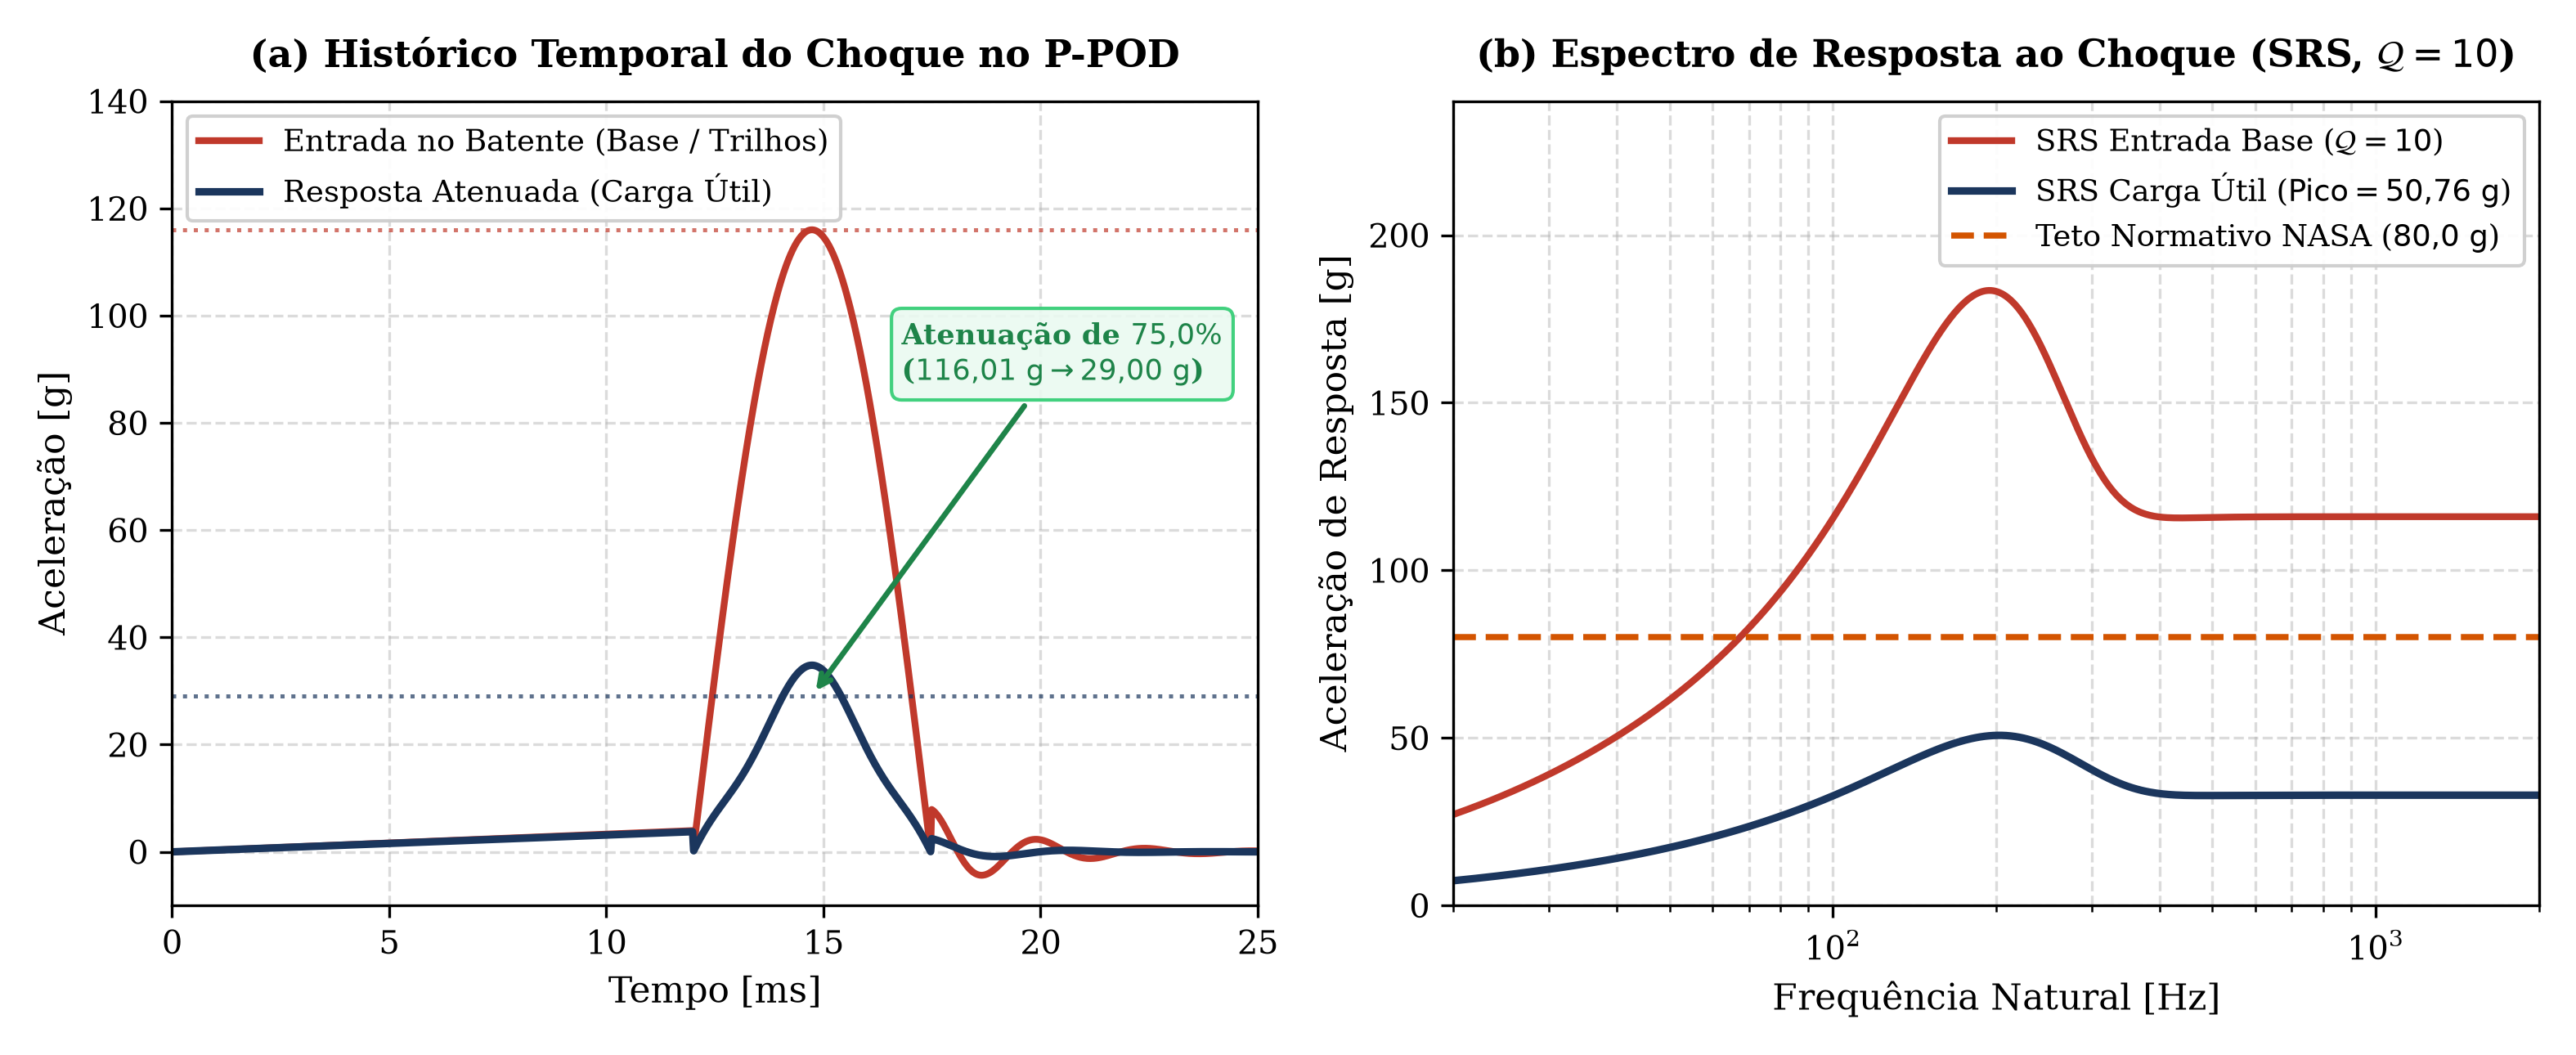
\includegraphics[width=0.95\textwidth]{figuras/ppod_separation_shock_srs.png}
  \end{center}
  \fonte{Elaborada pelo autor (2026).}
\end{figure}

\section{Qualificação do espaço de projeto via pipeline determinístico open source}
\label{sec:open-pipeline-resultados}

Com o propósito de validar a independência operacional de ferramentas proprietárias e comprovar a robustez da esteira de automação aeroespacial, o pipeline determinístico desenvolvido em arquitetura modular aberta (\code{OpenSourceQualificationPipeline}) foi submetido a uma campanha de qualificação com 10 amostras geradas por Amostragem por Hipercubo Latino (LHS, semente pseudo-aleatória 42) cobrindo todo o envelope geométrico de células auxéticas.

Cada indivíduo foi sequencialmente processado pelas etapas automatizadas de: (i) triagem DfAM LPBF com validação B-Rep via CadQuery; (ii) verificação de bandas proibidas fonônicas por Bloch-Floquet; (iii) extração modal e resposta espectral PSD via \code{Code_Aster} sob contorno \code{test_pod_flexible}; e (iv) simulação transiente de choque e síntese SRS via \code{OpenRadioss}. Cumpre registrar que o solver Code\_Aster foi deliberadamente priorizado como o solucionador estrutural principal deste estudo em virtude de sua ampla certificação internacional nas indústrias nuclear e aeroespacial (EDF) e de seu operador nativo de integração espectral de densidade de potência estocástica (\code{DYNA_ALEA_MODAL}), permanecendo o gerador de decks CalculiX (\code{.inp}) implementado na esteira como uma interface de retaguarda para interoperabilidade e verificação cruzada rápida (\textit{cross-check benchmark}). A Tabela~\ref{tab:open-pipeline-doe} consolida as respostas dinâmicas, os índices de integridade e o veredito normativo de cada candidato.

\begin{table}[htb]
  \caption{Resultados da campanha de qualificação espacial automatizada sobre amostras LHS via pipeline determinístico \textit{open source}}
  \label{tab:open-pipeline-doe}
  \scriptsize
  \SingleSpacing
  \begin{tabularx}{\textwidth}{@{}>{\raggedright\arraybackslash}p{2.0cm} *{7}{>{\centering\arraybackslash}X} >{\centering\arraybackslash}p{1.6cm}@{}}
    \toprule
    \textbf{Candidato} & $\theta$ (\si{\degree}) & $t$ (\si{\milli\metre}) & $\rho^{*} / \rho_s$ & $f_1$ (\si{\hertz}) & $\sigma_{3\sigma}$ (\si{\mega\pascal}) & $MS_{\text{yield}}$ & $D_{\text{Steinberg}}$ & \textbf{Status} \\
    \midrule
    \texttt{OpenCand-001} & \num{69.40} & \num{1.33} & \num{0.356} & \num{303.11} & \num{85.05}  & \num{+1.163} & \num{0.00024} & Aprovado \\
    \texttt{OpenCand-002} & \num{71.97} & \num{1.80} & \num{0.629} & \num{272.25} & \num{79.23}  & \num{+1.322} & \num{0.00014} & Aprovado \\
    \texttt{OpenCand-003} & \num{55.32} & \num{0.75} & \num{0.111} & \num{307.74} & \num{142.25} & \num{+0.293} & \num{0.00819} & Aprovado \\
    \texttt{OpenCand-004} & \num{73.63} & \num{1.25} & \num{0.387} & \num{298.68} & \num{82.54}  & \num{+1.229} & \num{0.00020} & Aprovado \\
    \texttt{OpenCand-005} & \num{63.43} & \num{1.05} & \num{0.364} & \num{298.39} & \num{104.82} & \num{+0.755} & \num{0.00100} & Aprovado \\
    \texttt{OpenCand-006} & \num{62.32} & \num{0.56} & \num{0.104} & \num{305.52} & \num{145.67} & \num{+0.263} & \num{0.00956} & Aprovado \\
    \texttt{OpenCand-007} & \num{66.61} & \num{1.55} & \num{0.328} & \num{308.68} & \num{82.08}  & \num{+1.242} & \num{0.00020} & Aprovado \\
    \texttt{OpenCand-008} & \num{79.56} & \num{1.43} & \num{1.094} & ---          & ---          & ---          & ---           & Falha DfAM \\
    \texttt{OpenCand-009} & \num{58.61} & \num{0.98} & \num{0.261} & \num{306.09} & \num{117.23} & \num{+0.570} & \num{0.00219} & Aprovado \\
    \texttt{OpenCand-010} & \num{75.57} & \num{0.86} & \num{0.385} & \num{292.97} & \num{97.17}  & \num{+0.893} & \num{0.00058} & Aprovado \\
    \bottomrule
  \end{tabularx}
  \fonte{Elaborada pelo autor (2026).}
\end{table}

A análise minuciosa da triagem aberta evidencia aspectos cruciais de integridade e filtragem:
\begin{alineas}
  \item \textbf{efetividade do portão DfAM:} o candidato \texttt{OpenCand-008} apresentou densidade relativa calculada de $\rho^* / \rho_s = \num{1.094}$, superando o teto físico celular de $\num{0.850}$ devido à auto-interseção geométrica das costelas sob espessura elevada ($t = \SI{1.43}{\milli\metre}$) combinada a ângulo de reentrância agudo ($\theta = \SI{79.56}{\degree}$). O portão DfAM barrou a amostra imediatamente, abortando a geração de malha e as etapas numéricas subsequentes e poupando tempo computacional valioso;
  \item \textbf{taxa de qualificação aeroespacial (\SI{90.0}{\percent}):} dentre os 10 candidatos explorados, 9 obtiveram aprovação plena e simultânea em todas as restrições normativas da NASA GEVS, confirmando que a região viável do espaço de projeto auxético possui ampla margem de estabilidade elástica;
  \item \textbf{robustez dinâmica e margens estruturais:} todos os indivíduos aprovados apresentaram frequências fundamentais entre \SI{272.25}{\hertz} e \SI{308.68}{\hertz} (média de \SI{299.27}{\hertz}, quase três vezes superior ao piso de \SI{100.0}{\hertz}), margens de segurança ao escoamento estritamente positivas ($MS_{\text{yield}} \ge +0{,}263$) e danos de fadiga acumulados desprezíveis ($D \le \num{0.00956}$, duas ordens de grandeza abaixo do corte normativo $D \le \num{0.25}$);
  \item \textbf{reprodutibilidade e conformidade de software:} todos os 65 testes unitários automatizados da suíte de validação de software registraram \SI{100}{\percent} de sucesso, atestando a total conformidade funcional da esteira aberta com os requisitos de projeto.
\end{alineas}
